%!TEX root = plos_template.tex
% Template for PLoS
% Version 1.0 January 2009
%
% To compile to pdf, run:
% latex plos.template
% bibtex plos.template
% latex plos.template
% latex plos.template
% dvipdf plos.template

\documentclass[10pt]{article}
%\documentclass[aps,twocolumn]{revtex4-1}
%\documentclass[aps,twocolumn]{article}

% amsmath package, useful for mathematical formulas
\usepackage{amsmath}
\setcounter{MaxMatrixCols}{50}
% amssymb package, useful for mathematical symbols
\usepackage{amssymb}

% graphicx package, useful for including eps and pdf graphics
% include graphics with the command \includegraphics
\usepackage{graphicx}

% cite package, to clean up citations in the main text. Do not remove.
\usepackage{cite}

\usepackage{color}

% Use doublespacing - comment out for single spacing
%\usepackage{setspace}
%\doublespacing

% Text layout
\topmargin 0.0cm
\oddsidemargin 0.5cm
\evensidemargin 0.5cm
\textwidth 16cm
\textheight 21cm

% Bold the 'Figure #' in the caption and separate it with a period
% Captions will be left justified
\usepackage[labelfont=bf,labelsep=period,justification=raggedright]{caption}

% Use the Science provided bibtex style
\bibliographystyle{Science}

% Remove brackets from numbering in List of References
\makeatletter
\renewcommand{\@biblabel}[1]{\quad#1.}
\makeatother

% Leave date blank
\date{}

\pagestyle{myheadings}
%% ** EDIT HERE **

\usepackage{bussproofs}

% xy-pic for diagrams
\usepackage[all]{xy}
% subcaption
\usepackage{subcaption}
% hyperref
%\usepackage[linkbordercolor={.67 .27 .27},citebordercolor={.09 .29 .54},urlbordercolor={.09 .29 .54}]{hyperref}
\usepackage{hyperref}
\hypersetup{colorlinks=true,
linkcolor=[rgb]{.67 .27 .27},
citecolor=[rgb]{.09 .29 .54},
urlcolor=[rgb]{.09 .29 .54}}

% color table cells http://goo.gl/ZmpJv
\usepackage[table]{xcolor}
% rotate text in table http://goo.gl/Lb4Zd
\usepackage{rotating}
% listings for code highlighting in appendix
\usepackage{listings}
\usepackage{setspace}
%!TEX root = ../plos_template.tex
% http://widerin.org/blog/syntax-highlighting-for-python-scripts-in-latex-documents
\definecolor{Code}{rgb}{0,0,0}
\definecolor{Decorators}{rgb}{0.5,0.5,0.5}
\definecolor{Numbers}{rgb}{0.5,0,0}
\definecolor{MatchingBrackets}{rgb}{0.25,0.5,0.5}
\definecolor{Keywords}{rgb}{0,0,1}
\definecolor{self}{rgb}{0,0,0}
\definecolor{Strings}{rgb}{0,0.63,0}
\definecolor{Comments}{rgb}{0,0.63,1}
\definecolor{Backquotes}{rgb}{0,0,0}
\definecolor{Classname}{rgb}{0,0,0}
\definecolor{FunctionName}{rgb}{0,0,0}
\definecolor{Operators}{rgb}{0,0,0}
\definecolor{Background}{rgb}{0.98,0.98,0.98}

\lstnewenvironment{python}[1][]{
\lstset{
numbers=left,
numberstyle=\footnotesize,
numbersep=1em,
xleftmargin=1em,
framextopmargin=2em,
framexbottommargin=2em,
showspaces=false,
showtabs=false,
showstringspaces=false,
frame=l,
tabsize=4,
% Basic
basicstyle=\ttfamily\small\setstretch{1},
%basicstyle=\ttfamily\footnotesize,frame=single,#1,
backgroundcolor=\color{Background},
language=Python,
% Comments
commentstyle=\color{Comments}\slshape,
% Strings
stringstyle=\color{Strings},
morecomment=[s][\color{Strings}]{"""}{"""},
morecomment=[s][\color{Strings}]{'''}{'''},
% keywords
morekeywords={import,from,class,def,for,while,if,is,in,elif,else,not,and,or,print,break,continue,return,True,False,None,access,as,,del,except,exec,finally,global,import,lambda,pass,print,raise,try,assert},
keywordstyle={\color{Keywords}\bfseries},
% additional keywords
morekeywords={[2]@invariant},
keywordstyle={[2]\color{Decorators}\slshape},
emph={self},
emphstyle={\color{self}\slshape},
%
}}{}

\usepackage{placeins}

% define colors
\definecolor{DeepRed}{rgb}{.82,.14,.16}
\definecolor{DeepBlue}{rgb}{0,0.36,0.62}

% set depth for table of contents
% http://tex.stackexchange.com/a/17879/6784
% http://tex.stackexchange.com/a/11669/6784
\setcounter{tocdepth}{4}
\setcounter{secnumdepth}{0}

%% ** EDIT HERE **
%% PLEASE INCLUDE ALL MACROS BELOW

% Set autoref text
% http://tex.stackexchange.com/a/36576/6784
\renewcommand*{\figureautorefname}{Fig.}
\renewcommand*{\equationautorefname}{Eq.}
\renewcommand*{\tableautorefname}{Table}

\renewcommand{\refname}{References and Notes}

\newcommand{\beginsupplement}{%
        \setcounter{table}{0}
        \renewcommand{\thetable}{S\arabic{table}}%
        \setcounter{figure}{0}
        \renewcommand{\thefigure}{S\arabic{figure}}%
     }
%% END MACROS SECTION


\begin{document}

% Add Figure, Table prefixes to references
% http://tex.stackexchange.com/a/6063/6784
\let\ref\autoref

% Table of contents
% http://tex.stackexchange.com/a/7357/6784
%\pagebreak
\pagenumbering{gobble}
\tableofcontents
\listoffigures
\listoftables
\pagebreak
\pagenumbering{arabic}

% Title must be 150 characters or less
\begin{flushleft}
{\Large
\textbf{Modularization of global genotype-phenotype mappings accesses a relative superset of biological functions}
}
% Insert Author names, affiliations and corresponding author email.
\\
Cameron Smith$^{1, \ast}$,
Ximo Pechuan$^{1}$,
Daniel Biro$^{1}$,
Aviv Bergman$^{1,2,3,4, \ast}$
\\
\bf{1} Department of Systems and Computational Biology,
\bf{2} Dominick P. Purpura Department of Neuroscience,
\bf{3} Department of Pathology, Albert Einstein College of Medicine, Bronx, NY, USA
\bf{4} Santa Fe Institute, 1399 Hyde Park Road, Santa Fe, NM 87501, USA
\\
$\ast$ E-mail: cameron.smith@med.einstein.yu.edu, aviv@einstein.yu.edu
\end{flushleft}

% Please keep the abstract between 250 and 300 words
\section{Abstract}
%!TEX root = ../plos_template.tex
Different gene regulatory network architectures are commonly thought to provide access to different collections of gene expression patterns that may ultimately result in different phenotypes~\cite{Alon2007}. The manner in which stochasticity in the gene expression process~\cite{Eldar2010,Sanchez2013} impacts the relationship between network architecture and the expression patterns each is capable of producing is not clear~\cite{Jothi2009,Chalancon2012}. In order to investigate this relationship, we begin with the finest grained notion of genotype to phenotype map, gene expression, and adopt a formalism to reason generally about probability distributions over such maps~\cite{Lane1998,MacLane1992,Awodey2006,Abramsky2011}. In all cases, this must be relative to a notion of network architecture, defined here as a hypergraph determining a hierarchical model~\cite{Lauritzen1996} over a given set of genes. We show that in a simple case where the highest-order gene regulatory interactions are allowed, then under some conditions the collection of accessible phenotypes is smaller than in some of the alternative cases in which only lower-order interactions are allowed. This conclusion is arrived at by comparing the geometries of spaces of probability distributions on genotype-phenotype maps for the case of a genome containing a given number of simultaneously interacting genes to the equivalent for all of the other possible gene regulatory network topologies on the same number of genes. We find that the latter spaces of probability distributions associated to the restriction to lower-order interactions are actually larger than the former one whenever the gene regulatory network topology contains a cyclic structure. A generalization of this result to an arbitrary number of genes implies that modularization of interactions, defined here as restriction from relatively higher- to lower-order interactions, within and among gene regulatory networks permits access to additional correlation patterns of expression among multiple interacting genes. That these additional gene expression patterns may enable the fulfillment of functional requirements in certain environments while remaining intrinsically inaccessible when highest-order interactions are allowed implies that, even when gene expression stochasticity is taken into account, network architectures may be functionally differentiated and thus serve as substrate for natural selection in a background of otherwise evolutionarily neutral space. The identification of \emph{interaction constraint}~\cite{Bar-Even2006,Johnson2010a} as an enabler as opposed to a limitation on accessible phenotypes may contribute to a more general explanation for the hierarchical modular architecture~\cite{Ravasz2002,Segre2005,Wagner2007,Erwin2009,Jothi2009,Bhardwaj2010,Colm} of the gene regulatory networks observed throughout the tree of life.


% Please keep the Author Summary between 150 and 200 words
% Use first person. PLoS ONE authors please skip this step.
% Author Summary not valid for PLoS ONE submissions.
%\section{Author Summary}
%%!TEX root = ../plos_template.tex
Several broadly applicable features of gene regulatory networks have been identified and experimentally validated to a reasonable level of confidence in the past few decades. Among these features are 1. stochasticity in the transcription process and 2. hierarchical modularity in gene regulatory network architecture. In this study, we consider explanations for the interplay between these two important features in a semi-formal model that considers both the developmental and evolutionary processes. We demonstrate within the context of our stylized model that the space of all possible gene expression patterns should be considered relative to a gene regulatory network architecture. Furthermore, we present a method that can in principle quantify these relationships for gene regulatory networks of arbitrary topological structure. This recognition derives from and has important future implications for the development of a constraint-based approach to characterizing the coevolution of stochasticity and hierarchical modularity and to modeling evolutionary processes more generally.


\section{Introduction}
%!TEX root = ../plos_template.tex
Probabilistic models of biological networks serve as a bridge between theory and experiment.  On the one hand, parameters in a probabilistic model can be fit to data obtained by measuring the levels of each variable. For example in gene regulatory networks, gene expression can be measured using microarray or sequence census methods \cite{Anastassiou2007,Friedman2008a,Zhang2013}.  On the other hand, one can model a biological network as a deterministic or stochastic reaction network which tracks levels of each molecule \cite{Alon2006,Voit2012}.  From the solution to this latter kind of model, one can then obtain theoretical predictions for the parameters of the probabilistic model in terms of reaction rates.  Comparison of the parameters fitted from data with the predicted values serves as a means for comparing theory with experiment and can serve as a starting point for improving the theory or for designing future experiments \cite{Tonsing2014}.

An important feature of experimental science is that it involves partial information.  In the course of a single measurement, one typically is not able to observe a biological network in its entirety.  Rather, one observes a subnetwork at a time and only obtains a more complete picture by later combining these partial views.  This contrasts with theory, where, one makes a representation of a closed system that provides explicit values for all quantities of interest.  In order for a probabilistic model to serve its purpose, it should also accomodate partial information and thus we will explicitly consider the effects of 1) carving out a subnetwork from its context and 2) coarse-graining observables. Observables representing partial information will generally arise in situations where a system is interacting with another system. This situation arises in the context of interpreting the potential existence of modular substructure within biological network data deriving from any given organism as well as with respect to the interactions between an organism and its environment.

% Studying this situation, we find that instances arise where the fact that a network context may interact with only partial information of the states of a given subnetwork can result in apparent inconsistency. Furthermore,

Inconsistency arises when a network context places more constraints on a subnetwork than it is capable of satisfying. The impact of this issue on genetic interactions has been considered previously in the context of population genetics \cite{EthanAkin389}. We exhibit a method of checking for such consistency and evaluating its likelihood of arising in the context of building probabilistic models of biological networks. When apparent inconsistency is observed, it must arise from the network context interacting with only partial information of the states of a given subnetwork. This would indicate that information about the network context must be included in order to maintain a consistent model of the system.

% Consider the case in which the network context is an environment placing independent and identical functional requirements upon a population of similar independent subnetworks and selecting for their architectures over many generations to satisfy those requirements. Our analysis of the probability of inconsistency arising relative to network architecture demonstrates that networks with a larger number of cycles are more likely to be subjected to inconsistent constraints that will be unable to be jointly satisfied. Since this probability of inconsistency is higher for networks with a larger number of cycles, this results in implicit selection against biological network architectures with a larger number of cycles. One would not expect such a bias to eliminate the existence of cycles in biological networks. However, it is reasonable to expect on the basis of this result a kind of hierarchical modularity: where modules that may possess cycles and are small relative to the overall size of the network exist within a globally hierarchical network structure. A similar problem has been considered previously in the context of population genetics \cite{EthanAkin389}. Of course, there are other factors which may contribute to the development of such network architectures. The evaluation of the hierarchical modularity property will require extensive future work, but its existence is consistent with many studies that have evaluated the architecture of various biological networks~\cite{Ravasz2002,Segre2005,Wagner2007,Erwin2009,Jothi2009,Bhardwaj2010,Chalancon2012,Colm}.

In \ref{sec:networkcontext} we describe the relationship between representations of biological networks and an abstraction of these referred to as network architecture that indicates the manner in which a subset of a network is connected to its context. We explain the connection between stochastic process models of biological networks and a generalization of the genotype-phenotype map applying to arbitrary biological networks referred to as \gnpm{} in \ref{sec:genenetworkphenmap}. \ref{sec:probabilitydistributionsonnetworks}--\ref{sec:inconsistency} contain examples of the underlying mathematical justification for our claims (more details of which are provided in \refsupp{}), and they can be skipped by readers who are primarily interested in the intuitive implications of our analysis. In \ref{sec:probabilitydistributionsonnetworks} we introduce the concept of network modules and define probability distributions over their states. \ref{sec:compatibilityofgpms} and \ref{sec:inconsistency} describe the different compatibility conditions that arise for different biological network architectures and demonstrate how these compatibility conditions lead to a set of inequalities determining a space of probability distributions for each network architecture. \ref{sec:cycliccontextunsatisfiableconstraints} and \ref{sec:probconstrgeometry} examine these constraints for the example of the three-cycle network architecture. \ref{sec:volrat} computes the likelihood of unsatisfiable constraints for all biological network architectures on four variables that possess cycles. Finally, \ref{sec:unsatisfiableconstrevolution} explains implications for the evolution of biological network architectures of the result that networks with a larger number of cycles are more likely to have unsatisfiable constraints placed upon them.

% We explain how one can pass from relatively fine-grained to more coarse-grained descriptions such as the ability to produce a given metabolite in a manner that is dependent upon interactions among multiple genes in \ref{secsupp:coarsegrainingphenotypes}. In \ref{sec:covergenotypespace} we define a biological network architecture as a collection of subsets of variables that together comprise a larger set. The different ways in which this is accomplished correspond to distinct BNAs.

% Traditional dynamical models of gene-regulatory networks begin by treating them as reaction networks whose known or hypothesized interactions are encoded by sigmoidal response functions \cite{Alon2006,Voit2012}. Genes that interact do so in such a manner as to either activate or inhibit one another leading to a dynamical model of the gene expression process.
% \begin{eqnarray*}
% {dg_i \over dt} =
% k_{is}  \prod_{j=1}^{N} \frac{k_{ija} g_j^{n_{ija}}}{1+k_{ija} g_j^{n_{ija}}}
% \frac{1}{1+k_{ijr} g_j^{n_{ijr}}} - k_{id} g_i
% \end{eqnarray*}
% for a network of $N$ genes where $g_i$s represent concentrations of gene products, $k_{ija}$s represent activation rates, $k_{ijr}$s represent repression rates, and $k_{id}$s represent degradation rates.
% The dual perspective is taken by probabilistic models whose parameters are fit to data obtained by measuring gene expression using microarray or sequence census methods \cite{Friedman2008a,Zhang2013}.
% In both of these classes of models, higher-order correlations are assumed to be accurately represented in terms of a sum over lower-order correlations.

% The evolution of \gnpm{} is an open question in biology. Specifically, how the higher level constraints imposed upon a system at a phenotypic level shape the elements and the interaction among the elements at a lower, genotypic level. Here we neglect the specific mechanisms by which one achieves such phenotypes and assume a statistical view of the observed phenotype. This communication introduces a framework that enable us to analyze how higher-level constraints, formulated in terms of probability of gene expression pattern might shape the allowable interactions among elements at a lower level.

% The genotype of an organism has a relatively straightforward definition in terms of the sequence of nucleotides comprising its genome. Phenotypes, on the other hand, can be described at different levels of organization~\cite{Dawkins1982,Stadler2001}. The concept of phenotype was initially defined at the level of macroscopically observable physical characteristics such as shape, size, color, and various combinations thereof~\cite{Johannsen1911}. However, since the advent of molecular biology, the lowest level description of phenotype might be considered to be the dynamic phenomenon that can be described by measuring the transcription states of all genes comprising an organism's genome. The time series that results from such observations can be used to infer various statistics that characterize gene expression such as correlations between pairs of genes. The statistics associated to any higher-level phenotype that is determined by a particular gene expression pattern should be functions of such statistics.

% % The present capability to observe phenotypes at various levels of organization raises several questions about \gnpm{}. One is how to define and characterize properties of the fundamental level of \gnpm{} that is embodied in the transcription process. Another is how to define and characterize the manner in which higher-order ``phenotype$_i$-phenotype$_{i+1}$'' mappings built on top of this one are affected by the properties of each of the levels existing below, and, on evolutionary timescales over which feedback may play a significant role, potentially also those above it.

% % We attempt to address these questions from an abstract perspective that is independent of the particular physical implementation of \gnpm{} in terms of complex networks of molecular interactions.
% We present a formal probabilistic description of the \gnpm{} that takes into account higher-order correlations among genes as well as evidence that gene expression is stochastic \cite{Swain2002,Paulsson2004,Thattai2004,Acar2008a,Lestas2010,So2011,Munsky2012,Neuert2013,Sanchez2013}. In order to assess the impact of these features on the evolution of gene regulatory network architecture, where architecture is here considered to be determined exclusively by observable correlations among genes \cite{Friedman2008a}, we use this description to precisely pose the question: For any genotype, given a space of probability distributions on the collection of \gnpm{}, does modularization of the genotype (restriction of correlations among genes, \refsupp{}) increase, decrease, or leave invariant the size of the accessible space of selectable gene expression patterns?
% % For example, if we have three genes that can all participate in a higher-order interaction (the highest-order among three genes being a trinary interaction) that generates a phenotype, but we restrict interactions to a lower-order subset consisting of all three possible binary interactions then this represents one particular way of modularizing over a given genotype (compare \ref{fig:conediagram}B top and middle).

% For those cases in which modularization results in no change to the space of probability distributions over \gnpm{} with respect to that defined on the full genotype (i.e. the single highest-order correlation referred to as non-modular), then there may be no method to select for one network architecture over another. On the other hand any differences in gene expression patterns that result from differences in network architecture may allow certain network architectures to be selected relative to one another. Here we show that those modularizations that introduce cycles into the gene-regulatory network architecture also expose the capacity for negative selection as a result of additional restrictions upon the gene expression patterns that apply to networks with cycles but not to those without.

% % then there would be no way to observationally distinguish the collection of possible gene expression patterns of organisms incorporating molecular mechanisms that explicitly impose such modularity, and thus no means of selecting specifically for modular or non-modular gene regulatory networks~\cite{Jothi2009,Colm}. If, on the other hand, modularization provides access to a larger or smaller space of probability distributions over \gnpm{} than for the non-modular case, then one can imagine that certain environmental conditions would be unable to be addressed by the functions capable of being achieved by the gene expression profiles accessible to one gene-regulatory network with respect to another. We provide a precise quantitative answer to the question stated above for several different modularizations over a collection of interacting genes.

% % In a network context in which all interaction orders are allowed, restriction of higher-order interactions within the underlying process intuitively reduces the size of the space of accessible gene expression patterns. However, in network contexts that are constrained to match the stationary structure of the underlying process, modularizations over a genotype that include at least one cycle in the hypergraph representing the resulting modular structure provide access to a \emph{larger} collection of potential gene expression patterns and thus a larger collection of potential biological functions that may derive from the expanded repertoire of such patterns. We provide a precise quantitative answer to the question stated above for several different modularizations over a collection of interacting genes.


% Results and Discussion can be combined.
% otherwise
% \section{Discussion}
% \section{Discussion}
\section{Results}
%!TEX root = ../plos_template.tex
\subsection{Coarse-graining gene expression admits a simple probabilistic model}
In any attempt to model gene regulatory networks, a focal subnetwork is conceptually carved out of a larger network context. The output of the subnetwork serves as input to the network context. The imposition of functional requirements by the network context upon the subnetwork is equivalent to requiring that certain patterns of output of the subnetwork be observable. The manner in which the subnetwork is connected to the network context determines the interactions that specify the structure of observations whereas the manner in which connections are made among genes within the subnetwork determine the structure of the process that underlies the repertoire of functions the network is capable of displaying independent of its context. It is from this perspective that we first motivate our model, by describing a simple representation of observing gene expression in a manner capable of mimicking the embedding of a given subnetwork within any possible network context.

\ref{fig:expression_concept}A shows a simplified representation of a bacterial chromosome or plasmid encoding a small gene regulatory network (GRN). The amount of a given transcript present in a cell given in terms of the discrete counts obtained via sequence census methods (e.g. RNA-seq) or relative abundance derived from microarray data can be binned into a smaller number of discrete classes by setting a collection of thresholds on the original data set. If only a single threshold is given, then the data can be binned into two classes depending upon whether or not the original measurement surpasses the given threshold \ref{fig:expression_concept}B. If a large enough number of thresholds is available to distinguish among all possible molecule counts, then this observational protocol becomes complementary to mechanistic models of stochastic gene expression that seek solutions of the master equation, which contain probability distributions over molecule counts \cite{Walczak2009,Mugler2009}. At the lowest-level of the genotype-phenotype mapping, these coarse-grained expression values can be viewed as collectively determining the lowest level in the aforementioned hierarchy of phenotypes. In this way, the data derived from a number of samples of a given network can be described using binary sequences \ref{fig:expression_concept}C. For a given number of genes, it is possible to sample any subset of genes and the structure of this sampling process plays a role in determining the interpretation of the structure of the underlying process that generates the data, which, in this case, includes all regulatory elements that impinge upon the GRN module under consideration. For example, if, whenever we sample, we always consider the expression state of three out of three genes, we imply that the underlying process can be represented as a joint probability distribution over those three genes \ref{fig:expression_concept}C top. If instead we consider each pair of genes separately \ref{fig:expression_concept}, we imply the existence of a different kind of structure, which is the sum or union of several simpler spaces of probability distributions, each representing lower order interactions within the network that has been conceptually carved out of a larger network context.

\subsection{Divergence between observational structure and the structure of the underlying process driving gene expression can lead to inconsistency}
We can use an undirected graph (e.g. \ref{fig:inconsistentthreecycle}A, bottom left) to indicate interactions allowed by various GRN architectures (GRNAs). Each node of the graph is associated to the probability distribution that specifies probabilities for each gene to be observed in each of the states specified by the coarse-graining process described in the previous section. Each edge of the graph specifies a joint probability distribution for both of the nodes it contains (or connects) to simultaneously take on a given pair of values. We generalize this in what proceeds to hypergraphs where each edge can contain an arbitrary number of nodes. In this context it is presumed that via marginalization the probability distributions associated to each edge are consistent with the probability distributions associated to each node. This description is similar to that of a Markov Random Field (a particular type of graphical model defined over undirected graphs) as a model for the stationary distribution of the stochastic process underlying gene expression \cite{Lauritzen1996,Chen2013a}. However, the implication of existence of a factorizable joint probability distribution over all nodes in the graph, which is implicit in the machine learning interpretation of graphical models, is not assumed here (Supplementary Material) \cite{Barber2012,Bishop2007,Murphy2012,Koller2009}.

\ref{fig:inconsistentthreecycle}A provides a concrete example where we assume three genes interact via all possible pairwise combinations and that via the coarse-graining process we have binned the expression state of each gene into one of two classes. Note that this graphical model is completely general and we can have, in principle, an arbitrary number of genes and an arbitrary number of classes in the assignment of expression states up to the maximal resolution of the method by which the observations are performed. Each node of the graph in \ref{fig:inconsistentthreecycle}A represents a probability distribution over the observation of each gene in either of the two states established in the coarse-graining process, which for node three are given by $p((3 \mapsto 0,\,\, 3 \mapsto 1))=(0.5,0.5)$. Given an edge we consider a map or function that takes as input the two genes connected by or contained within that edge and maps those two genes simultaneously to the available expression states. For example in \ref{fig:inconsistentthreecycle}A bottom there are maps $12 \mapsto 11$, $23 \mapsto 10$, and $31 \mapsto 10$ with associated probabilities $p(12 \mapsto 11)=0.1$ \ref{fig:inconsistentthreecycle}A top purple box and bottom purple arrows, $p(23 \mapsto 10)=0.1$ \ref{fig:inconsistentthreecycle}A top orange box and bottom orange arrows, and $p(31 \mapsto 10)=0.1$ \ref{fig:inconsistentthreecycle}A top green box and bottom green arrows. Each of the probability tables adjacent to each edge in the graph in \ref{fig:inconsistentthreecycle}A assigns a probability distribution to a set of the maps from the nodes connected by the edge to all possible combinations of the expression states. As these maps take collections of genes as input and produce collections of expression states as outputs we refer to them as genotype-phenotype mappings and thus to the associated probability distributions as probability distributions over genotype-phenotype maps.

If the probability distribution in \ref{fig:inconsistentthreecycle}A represents the actual structure and particular parameters of the process generating the gene expression data, we can also consider the problem of inferring the parameters of a hierarchical model (Supplementary Material) for the probability distribution specified adjacent to the nodes and edges of the graph given the assumption that the structure of a given GRN is modeled by a given graph and then observe the GRN according to that assumption. \ref{fig:inconsistentthreecycle}B top left represents data containing three hundred observations generated by a process whose structure is equivalent to that of \ref{fig:inconsistentthreecycle}A except that we consider the case in which each expression state is equally likely. We now use maximum likelihood estimation \cite{Barber2012} to detertmine the parameters of a model like that of \ref{fig:inconsistentthreecycle}A given the dataset in \ref{fig:inconsistentthreecycle}B top left. \ref{fig:inconsistentthreecycle}B top middle shows that indeed all possible binary sequences representing the expression states for genes one, two and three are approximately uniformly represented in the given samples and the green bars in \ref{fig:inconsistentthreecycle}B bottom show the marginals of this joint distribution. Alternatively, we can infer the marginal probabilities using the sum-product (belief propagation) algorithm \cite{Barber2012} resulting in the yellow bars in \ref{fig:inconsistentthreecycle}B bottom. If we perform the same sequence of steps on the data in \ref{fig:inconsistentthreecycle}C top left, only the (loopy) belief propagation algorithm returns marginal distributions (\ref{fig:inconsistentthreecycle}C bottom) that are consistent with the data. This is a result of the fact that no joint probability distribution having these empirical marginals exists and maximum likelihood estimation determines a joint distribution that only approximates the empirical marginals. Dually, only the data of \ref{fig:expression_concept}C bottom and not that of \ref{fig:expression_concept}C top is consistent with the probabilities represented in \ref{fig:inconsistentthreecycle}A.

This inconsistency is a result of the fact that the network architecture in \ref{fig:inconsistentthreecycle}A contains a cycle \cite{Lauritzen1996,Geiger2006,Wainwright2007} and that we have given an ostensible data set and thus parameters that lead to the impossibility of constructing a consistent joint probability distribution over all three genes. For the case of the architecture in \ref{fig:inconsistentthreecycle}A, and moreover for any GRNA of any size that contains one or more cycles, the possibility of finding a joint distribution over all genes requires the implicit assumption that the structure of the generating process can be viewed simultaneously as that of \ref{fig:expression_concept}C top and that of \ref{fig:expression_concept}C bottom. The spaces of probability distributions associated to the two GRNAs contrasted in \ref{fig:expression_concept}C are different. This situation leads to the question of whether or not it is possible to classify the geometries and thus relationships among the spaces of probability distributions associated to all possible GRNAs on a given number of genes.

\subsection{Gene-regulatory network architecture is associated to the geometry of spaces of probability distributions over genotype-phenotype maps}
The collection of all possible GRNAs in the context of hierarchical models is equivalent to the lattice of all possible reduced subsets of genes (Supplementary Material). For example, \ref{fig:conediagram}A contains the lattice of reduced subsets of three genes. We are only interested in those subsets that contain at least one copy of each gene, which corresponds to the region highlighted with a gray background in \ref{fig:conediagram}A. Each GRNA induces a different structure on the genotype-phenotype maps underlying it. For example, \ref{fig:conediagram}B shows in the same vertical order the different structures induced by the three architectures highlighted in green in \ref{fig:conediagram}A.

We consider those GRNAs found lower in the lattice of \ref{fig:conediagram}A to be of higher modularity because each corresponds to the increasing restriction from higher- to lower-order interactions among genes and thus the restriction of simultaneous evaluation of phenotypes over the collection of genes. \ref{fig:conediagram}B top corresponds to the least modular GRNA because phenotype values are assigned simultaneously to all three genes. \ref{fig:conediagram}B middle exhibits an elevated degree of modularity because phenotypes are only simultaneously assigned to pairs of genes despite the fact that on timescales longer than that fundamental to the generating process it is possible to measure the phenotype values of all three genes simultaneously. Similarly, \ref{fig:conediagram}B bottom is even more modular because phenotype values are only assigned to one gene at a time. The structure of these GRNAs is associated to coverings of genotype space in the Supplementary Material.

Each of the GRNAs in \ref{fig:conediagram}A can be associated to a space of probability distributions over genotype-phenotype mappings. \ref{fig:conediagram}C schematically depicts the relationships among the probability distributions associated to the corresponding architectures and genotype-phenotype mappings in \ref{fig:conediagram}B. The inconsistency noted in the previous section between the architectures \ref{fig:conediagram}B top and middle is a result of the differing geometries in \ref{fig:conediagram}C middle. There, the smaller darker gray region corresponds to the space of all possible probability distributions for all possible parameters achievable via application of the linear transformation corresponding to marginalization to the probability distribution defined over all possible genotype-phenotype mappings associated to the network architecture in \ref{fig:conediagram}B top. Similarly, the lighter gray region corresponds to the analogous structure for \ref{fig:conediagram}B middle.

This relationship indicates that there are certain cases in which a given GRNA exhibiting a relatively higher degree of modularity nevertheless provides access to a larger space of possible probability distributions and thus of correlations among genes which can be coarsely referred to as gene expression patterns. These patterns may serve as substrate for natural selection of GRNAs with particular functions by the network context within which the small modules we have considered so far function.

\subsection{Some GRNAs provide access to different collections of gene expression correlations}
Relationships between spaces of potential gene expression patterns like that of \ref{fig:conediagram}C middle occur for all GRNAs on any number of genes so long as there exists at least one cycle in the corresponding network architecture. For the case of three genes, there is only one class of graphs containing a cycle, which is that of \ref{fig:conediagram}B middle. For the case of four genes there are nine different classes of graphs containing cycles and these nine classes can be split into two groups depending upon whether or not the edges of the graphs are each restricted to contain only two genes (2-uniform hypergraphs, which are equivalent to undirected graphs). \ref{fig:non2uniformcyclichypergraphhasse} shows the components of the lattice analogous to that of \ref{fig:conediagram}A containing the five out of the nine isomorphism classes of hypergraphs on four genes that have cycles but that are not 2-uniform (the hypergraphs where at least one edge has more than two genes).

Given this larger collection of GRNAs with cycles we can assess the relative sizes of the analogs to the light and dark gray spaces (\ref{fig:conediagram}C middle) of probability distributions over genotype-phenotype maps. We assess the likelihood of choosing a point in the dark gray region at random by computing the ratio of the volume of the dark gray region (associated to the non-modular GRNA analogous to that of \ref{fig:conediagram}B top with a single edge containing all four genes), whose architecture and thus volume is fixed, to that of the light gray region, whose volume varies according to each of the cyclic graphs associated to a GRNA on four genes. We refer to this number as the non-modular:modular volume ratio or~$\frac{\text{Vol}(\mathbb{M}(\mathcal{G}))}{\text{Vol}(\mathbb{L}(\mathcal{G}))}$~(Supplementary Material). \ref{fig:ncycvolrat}A shows the relevant computations for seven different graphs where the edges are restricted to each contain two genes. The spaces are equivalent and thus the volume ratio equal to one for graphs lacking cycles (e.g. the first three graphs along the $x$-axis of \ref{fig:ncycvolrat}A). For the four network architectures in \ref{fig:ncycvolrat}A containing cycles, the volume ratio is consistently less than one. This quantifies the degree to which the space of probability distributions associated to the network architecture depicted along the $x$-axis is larger than the space of probability distributions associated to the non-modular architecture.

\subsection{Over evolutionary timescales network context can impose constraints on network architecture via the requirement of particular expression patterns}

The difference in the repertoires of gene expression patterns available to the various architectures with cyclic components each with respect to the structure corresponding to the joint distribution over all genes is equivalent to the statement that certain probability distributions over genotype-phenotype maps are only accessible from a certain class of GRNAs. This indicates that if the context (see \ref{fig:stochdynscheme} left) within which the network modules we have considered so far are embedded places certain functional requirements upon them, then the ability of any GRN to be able to meet those requirements must be considered relative to the geometry of its associated space of probability distributions. The ability to access certain correlation patterns is also dependent upon the network context.

For those GRNAs containing cycles, there are certain functional requirements that can be achieved so long as only local and not global consistency is required of them (Supplementary Material). Once global consistency is imposed as in the structure corresponding to the joint distribution over all genes, those functions that were accessible when only local consistency is imposed will become unavailable. This observation suggests a mechanism by which the GRNA may be imposed upon a collection of genes. \ref{fig:stochdynscheme} right shows a schematic of one potential scenario. The black dots in the center represent an initial condition of a stochastic process that is selected for its ability to achieve one of two different stationary distributions represented by the blue and the red dots respectively. The architecture whose space of probability distributions is represented in the top row of \ref{fig:stochdynscheme} is however unable to precisely achieve as its stationary distribution the point represented by the red dot in the bottom row of \ref{fig:stochdynscheme}.

When selective pressure is induced equivalent to the distribution located at the blue dot, either of the architectures are essentially equivalent with respect to the statistics of samples from their corresponding probability distributions and they can thus be considered as members of an evolutionarily neutral space. On the other hand, selective pressure equivalent to the collection of probability distributions located at the red point differentiates between the networks of the top and bottom row or equivalently between the network of the bottom row when global consistency is imposed versus the same network when only local consistency conditions are imposed. The same qualitative relationship holds true for the spaces of probability distributions of all GRNAs of any size and for any number of different expression levels so long as the graph associated to the space of probability distributions contains at least one cycle.


\section{Discussion}
%!TEX root = ../plos_template.tex
To contribute to the broader goal of establishing an integrated framework that synthesizes hypothesized intrinsic and extrinsic constraints necessary to understand the functioning and evolution of biological systems, here we have attempted to trace a path from relationships among spaces of probability distributions to their impact upon stochastic models of gene regulatory networks and, via the impact of gene expression on phenotypes, to evolutionary processes. One goal of measuring gene expression at transcriptomic scale has to be to uncover the structure of the generative process encoded in the GRN interactions involved, but, so far, even the most sophisticated methods of describing them at the mechanistic level are only solvable for extremely simple regulatory network architectures~\cite{Walczak2009,Mugler2009}. This fact has, in part, motivated computational biologists to develop a large collection of algorithms to infer aspects of this structure~\cite{DeSmet2010} and experimental biologists to compare networks on the basis of their hierarchical and modular architecture~\cite{Ideker2012}. Our model and its framework put forward a class of fundamental constraints, that while not unique to gene regulatory networks, must nevertheless impact their structure at the level of abstraction described here. The fact that GRNA impacts the structure of the entire space of probability distributions over genotype-phenotype maps---and not just a parameter-dependent fragment of it---accessible to each given architecture provides a clear mechanism by which natural selection may mold GRNAs.

It is clear that in most cases, when gene regulatory networks are studied, we remove a subnetwork from a larger context~\cite{Alon2007}. In our case, the network context, such as that schematized in \ref{fig:stochdynscheme}A, must play a crucial role, in addition to the subnetwork architecture upon which we have focused here, in determining whether or not it is possible to access the gene expression patterns that more highly modular regulatory network architectures ostensibly provide access to. One mechanism by which the network context may determine access to correlations that lie outside what is achievable in the non-modular case is via a form of cis-regulation that enables the breakage of statistical dependence in a time-dependent manner. On the other hand, some forms of epigenetic regulation may serve the opposite purpose to couple genes which do not otherwise interact. It will be important in future work to address these questions in the context of developing bottom-up stochastic process models that allow for the explicit encoding and solution of more complex gene regulatory networks~\cite{Walczak2009,Mugler2009}, which also allow for the incorporation of the effects of epigenetic regulation. Our results suggest that when requirements such as that in \ref{fig:inconsistentthreecycle}A are placed upon a network, then the network context must ultimately serve to decouple statistical dependency intrinsic to the network architecture, and this essentially requires the type of hierarchical relationship implicit in that among genetic and epigenetic regulation but also to that within hierarchically organized transcription factor networks \cite{Jothi2009,Bhardwaj2010,Chalancon2012,Colm}.

% In biology, as in other sciences such as physics~\cite{Gell-Mann1956}, prevailing wisdom suggests that anything is allowed unless it has been demonstrated to some reasonable degree of confidence to be forbidden. We suspect that there are many other simple physical and mathematical constraints that can be brought to bear on biological problems. Constraint-based models that extract invariants of metabolic and other biochemical reaction networks provide a shining example of this approach~\cite{Karp2012,Bordbar2014}. The use of fundamental constraints to characterize geometric properties of phenotype space have begun to elicit applications of this approach to evolutionary processes~\cite{Shoval2012,Sheftel2013,Jordan2013}. At first, statements of such may only be effective at a relatively high level of abstraction. However, as a larger number of broad constraints are organized and integrated into a common language they can be applied to increasingly detailed models that integrate omic scale information over developmental and evolutionary timescales~\cite{Gunawardena2013}. Approaches of the type we have exhibited here hold promise for realizing the tremendous potential that continues to be built up in databases of high-throughput genomic data.

The ultimate goal of constraint-based approaches toward understanding molecular interaction networks should be to develop a theory capable of expressing the manner in which information is stored and transmitted in networks of molecular interactions~\cite{Tkacik2011a,Bialek2012} and how such processes produce the higher-order properties such as phenotypes that serve as substrate for natural selection~\cite{Mora2013}. Subtle but essential developments in information theory and its applications makes connections between molecular networks~\cite{Cheong2011,Brennan2012} and networks of neurons immediate~\cite{Stanley1999,Balduzzi2008,Balduzzi2009,Balduzzi2012}, while also supporting generalization from molecular networks to organisms and their populations in application to evolutionary processes~\cite{Kussell2005a,Rivoire2011}. Common to all of these instantiations is the drive toward understanding the manner in which relationships between some interacting entities and the mutual constraints implicit to such interactions can be represented mathematically in both algebraic and geometric form. While this study has provided another instantiation of such an approach, it seems to be a mere fragment of a deeper theory requiring expression in terms of a language that curious specialists from each of the relevant fields can all understand well enough to speak.


% This section is often entitled "Materials and Methods"
% You may title this section "Methods" or "Models".
% "Models" is not a valid title for PLoS ONE authors. However, PLoS ONE
% authors may use "Analysis"
\section{Methods}
%!TEX root = ../plos_template.tex
Details of the models and methods are provided as Supplementary Material.


% Do NOT remove this, even if you are not including acknowledgments
\section{Acknowledgments}
%!TEX root = ../plos_template.tex
Support was provided by MSTP training grant T32-GM007288 to CS. The authors thank Jay Sulzberger for sharing important discussions and mathematical insight. We thank Noson Yonofsky and Andrew Yates for helpful discussions.


%\section{References}
% The bibtex filename
\bibliography{bib/books,bib/papers}

\pagebreak
\section{Figure Legends}
%!TEX root = ../plos_template.tex
\begin{figure}[!ht]
\centering
\noindent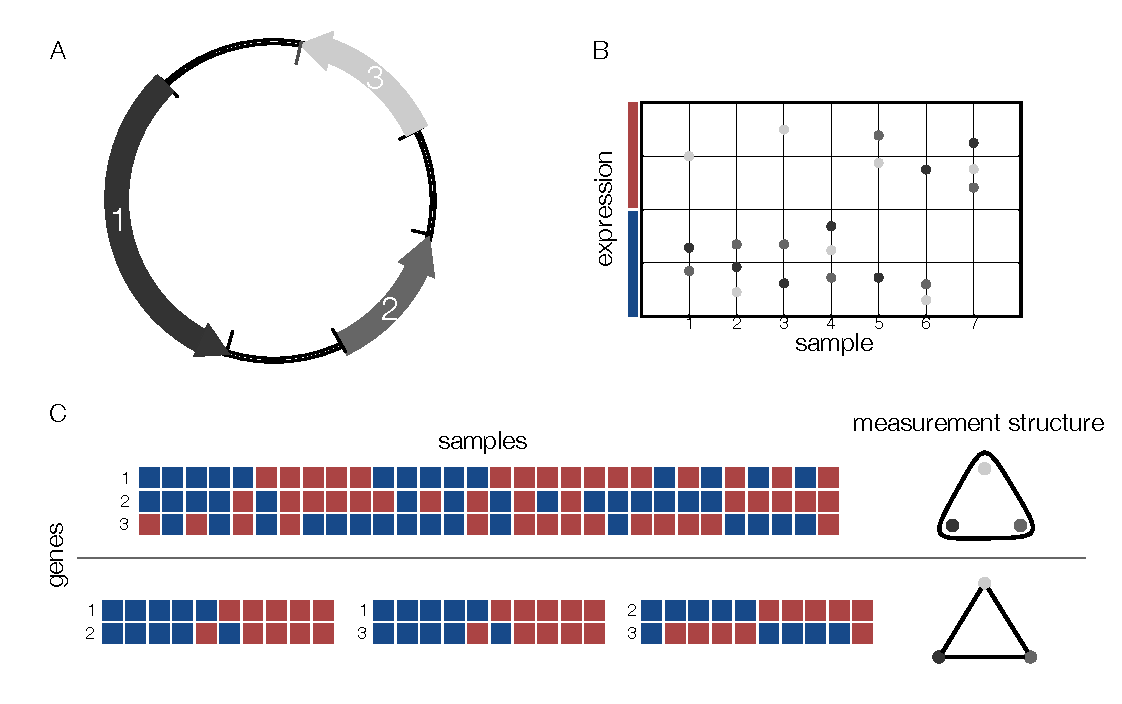
\includegraphics[width=0.9\columnwidth]{fig/figure_expression_concept.pdf}
\caption{{\bf Coarse-graining of gene expression data.} (A) Minimal representation of a small GRN consisting of three genes encoded in a plasmid. (B) Example binary coarse-graining of gene expression data. For each sample a measurement is taken for all three genes. The expression levels are binned into one of two classes represented by the red and blue bars representing relatively high and low expression respectively. (C) Heat map representation of coarse-grained gene expression data under the assumption of two different GRNAs. The samples on top and the associated measurement structure correspond to the standard method of measurement where it is assumed that the structure of the underlying network can be represented by a joint probability distribution over all genes. The bottom represents data collected under the assumption of an alterantive GRNA where only binary interactions between each pair of genes are presumed to be necessary to explain the gene expression patterns capable of being produced.}
\label{fig:expression_concept}
\end{figure}

\begin{figure}[!ht]
\centering
\noindent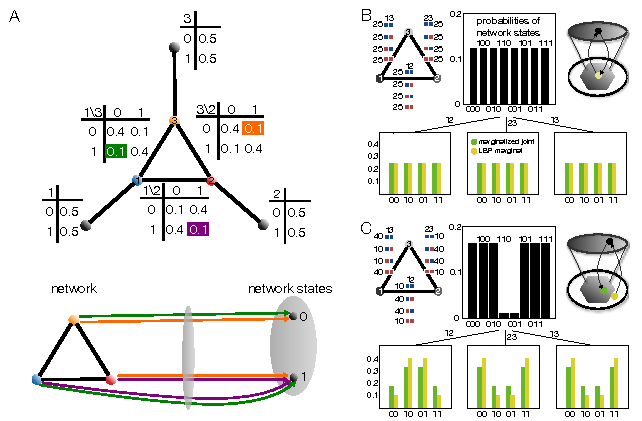
\includegraphics[width=0.9\columnwidth]{fig/inconsistentthreecycle.pdf}
\caption{{\bf Graphical model of inconsistent gene expression data.} (A) An example graphical model structured according to \ref{fig:expression_concept}C bottom. The graph contains three nodes each representing one of the genes depicted in \ref{fig:expression_concept}A. The gray node coming from each node is placed next to the node marginal distribution depicted in the associated table. The edge marginal distributions are placed along the edges. The colored boxes (top) are associated to the genotype-phenotype mappings represented by the equivalently colored arrows (bottom). The phenotype values derive from the coarse-graining process over gene expression data depicted in \ref{fig:expression_concept}B. (B) Given the graphical model in panel A, the top-left panel represents three hundred samples comprising a data set consistent with a uniform distribution over all genotype-phenotype maps. The top-middle panel represents the joint probability distribution determined via maximum-likelihood estimation on the sufficient statistics given in the top-left panel. The green bars in the bottom three panels represent the marginalization of this joint distribution according to the structure of the graph. The yellow bars in the bottom three panels represent the marginal distributions determined via the sum-product algorithm (loopy belief propagation). The top-right panel is a schematic where the top gray ellipse represents the space of joint probability distributions on three genes each with two expression states (i.e. $\Delta_7$: the eight-dimensional probability simplex) and the bottom ellipse represents the union of three copies of the four-dimensional probability simplex (i.e. $\Delta_3^{\oplus 3}$), one for each edge in the graph.  For this data, maximum likelihood estimation and loopy belief propagation yield equivalent points in $\Delta_3^{\oplus 3}$ and therefore the distance separating them is $0$. (C) Same as B, but with data consistent with \ref{fig:expression_concept}C bottom and, equivalently, the node and edge marginal distributions in panel A of this figure. For this data, maximum likelihood estimation and loopy belief propagation yield different points in $\Delta_3^{\oplus 3}$ so the distance separating these two collections of distributions is greater than $0$.}
\label{fig:inconsistentthreecycle}
\end{figure}

\begin{figure}[!ht]
\centering
\noindent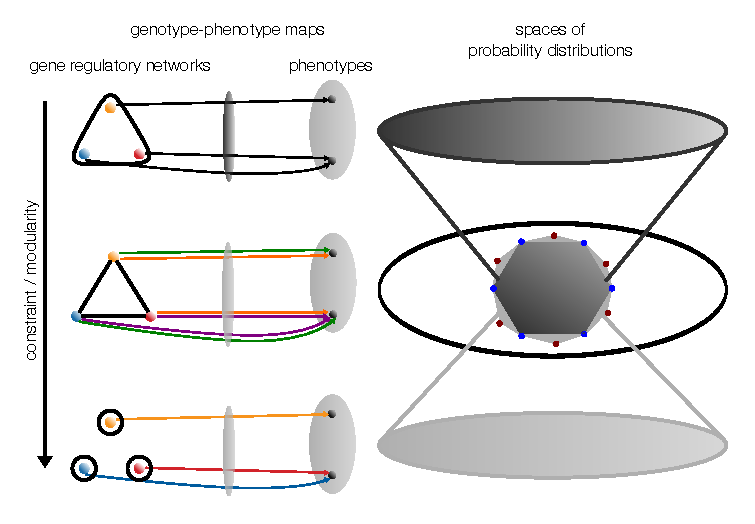
\includegraphics[width=0.9\columnwidth]{fig/conediagram.pdf}
\caption{{\bf Relationship between gene regulatory network models and spaces of probability distributions.} (A) The collection of all possible GRNAs over three genes forms a lattice represented here by its Hasse diagram. An analogous lattice of GRNAs exists for any number of genes. The Hasse diagram shows the manner in which GRNAs are hierarchically related and are thus able to be embedded within one another. (B) Explicit examples of genotype-phenotype mappings over three GRNAs from panel A highlighted in green are represented as arrows mapping the genes represented as nodes of the graph underlying the GRNA into the collection of phenotype values determined by the coarse-graining chosen in \ref{fig:expression_concept}B. There is a different collection of possible genotype-phenotype mappings depending upon the structure of the GRNA. (C) Each collection of genotype-phenotype maps one representative for each GRNA depicted in panel B is associated to a space of probability distributions defined over it. Moreover, the spaces of probability distributions associated to each graph are related via marginalization maps. The top represents a joint probability distribution which can be marginalized to the middle space which in turn can be marginalized to the bottom space. The light gray polytope in the middle represents the space of distributions consistent with the marginalization map from the middle to the bottom. The dark gray polytope represents the space of probability distributions consistent with marginalization from the top to the middle.}
\label{fig:conediagram}
\end{figure}

% \begin{figure}[!ht]
% \centering
% \noindent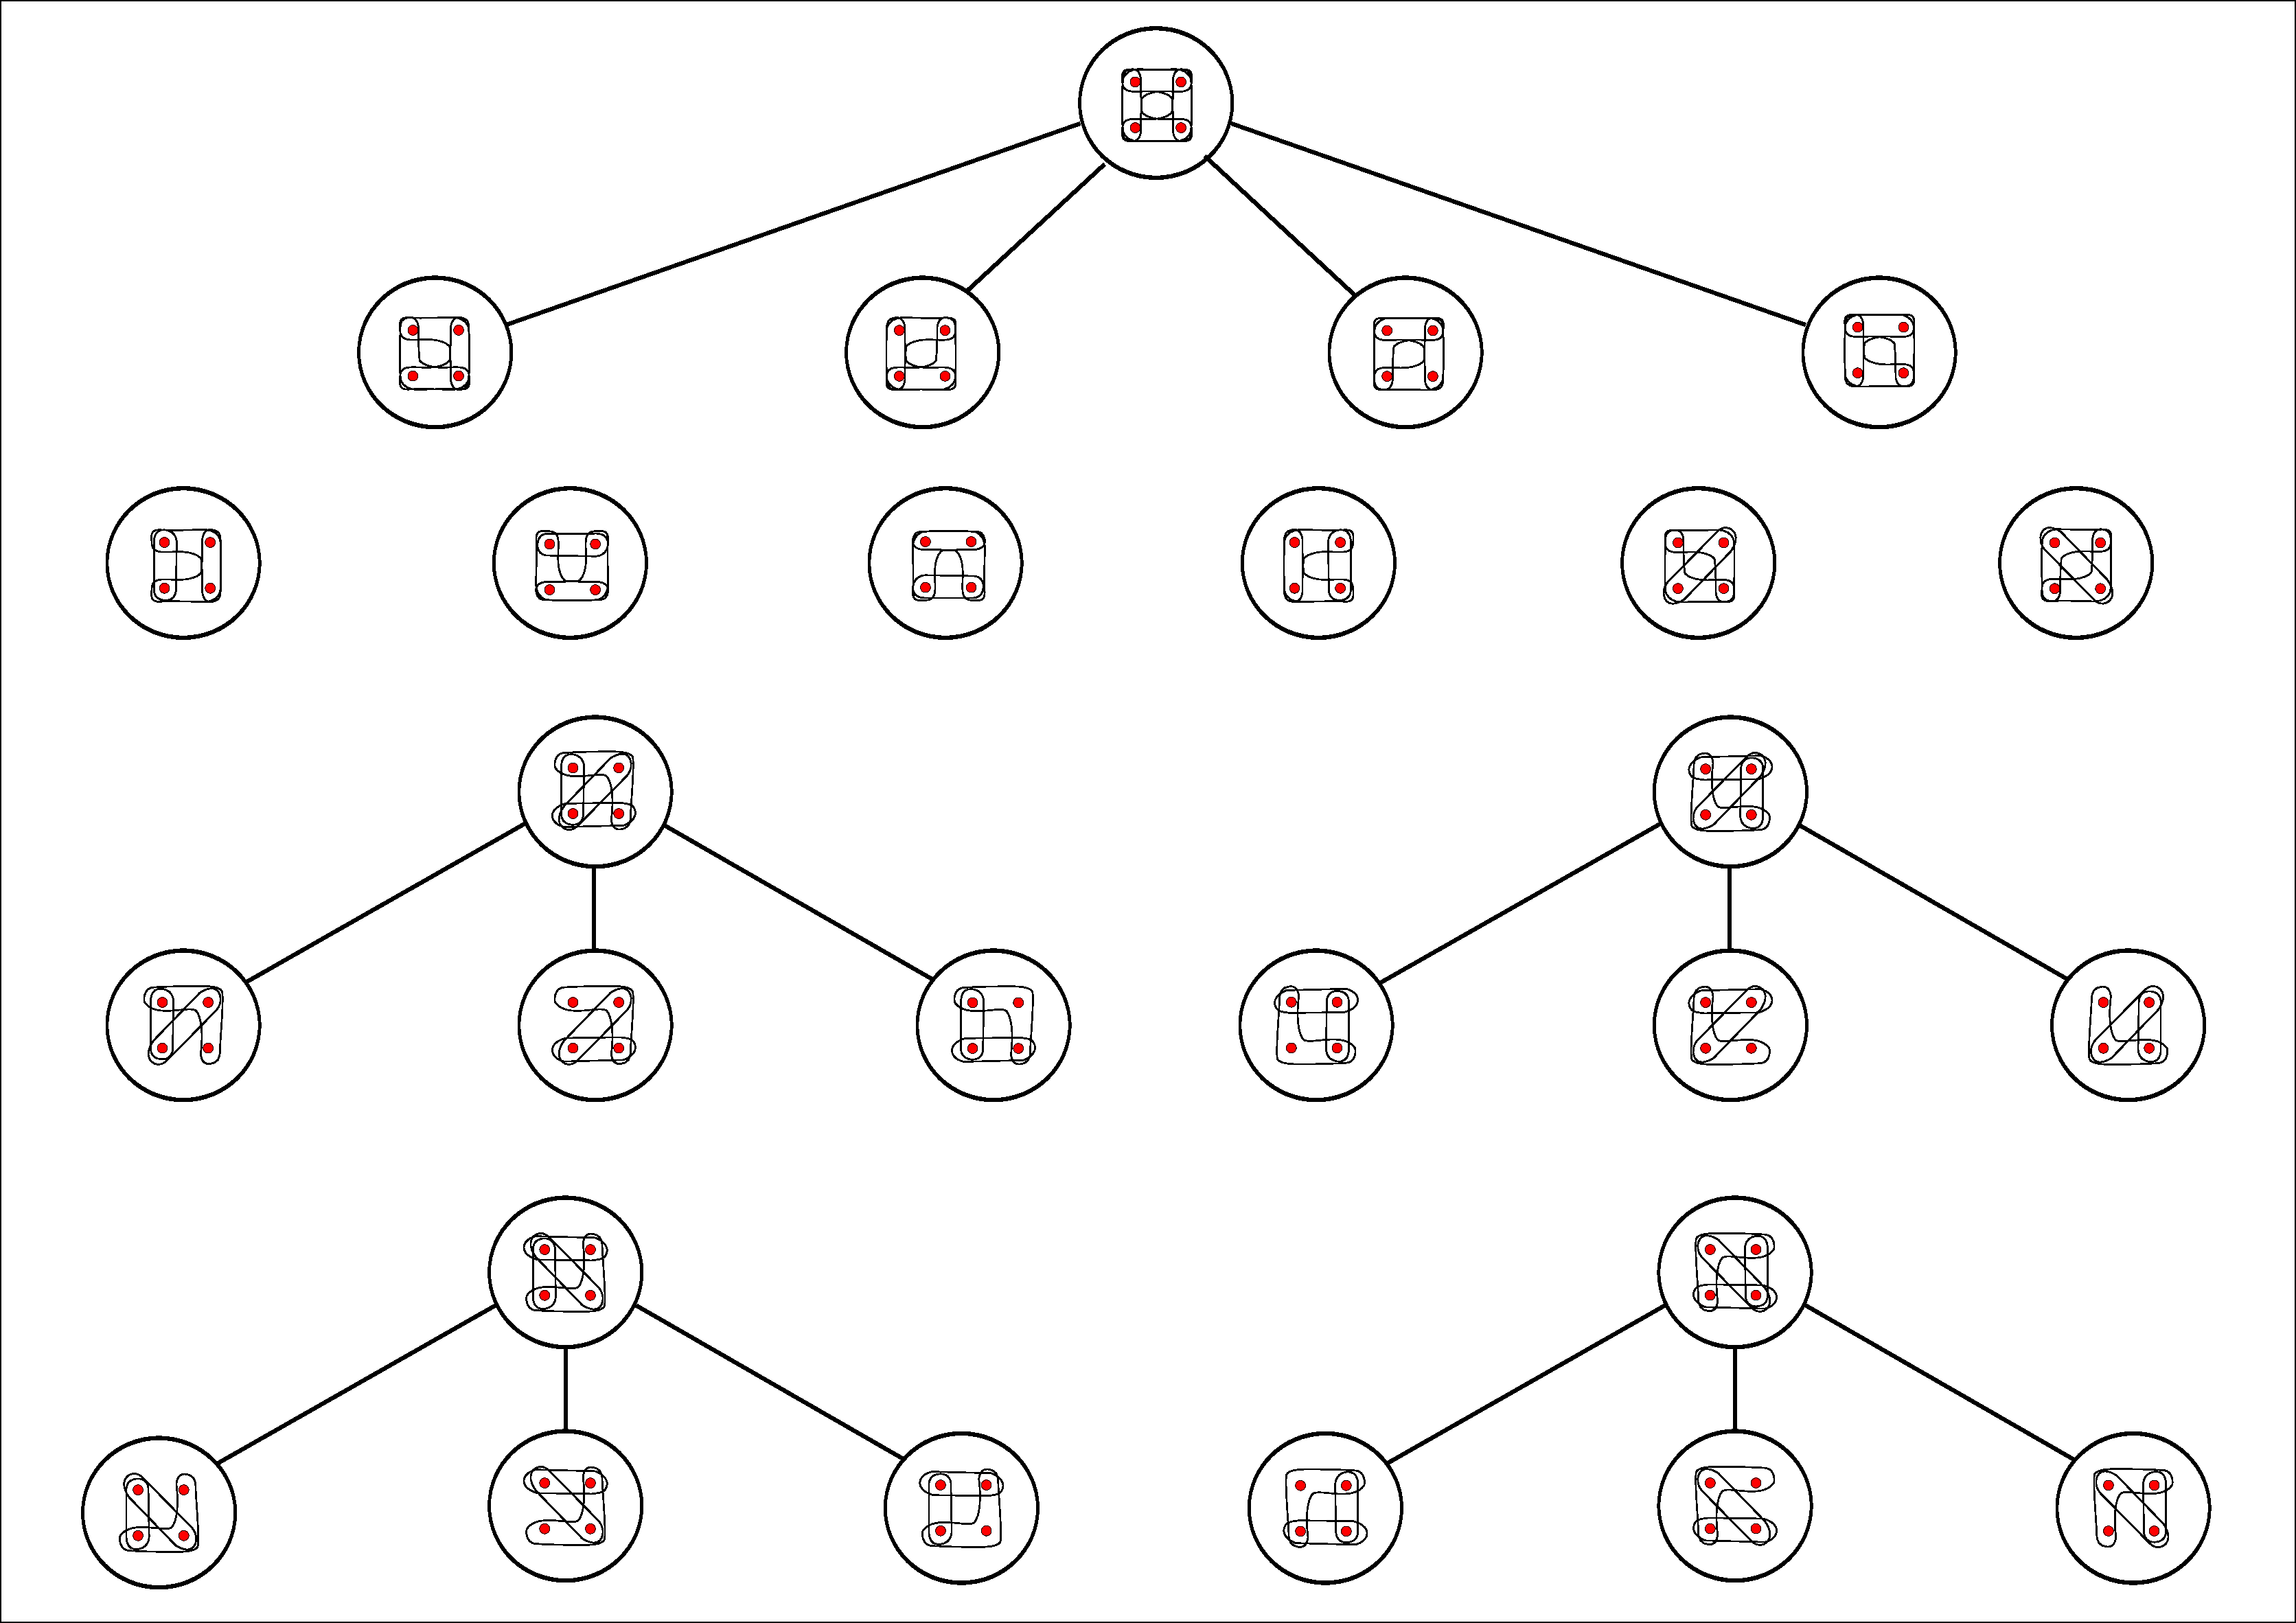
\includegraphics[width=1.0\columnwidth]{fig/non2uniformcyclichypergraphhasse.pdf}
% \caption{{\bf Hierarchical relationships among all possible classes of hypergraphs that are not graphs (i.e. not 2-uniform) but have cycles.} (A) There is a Hasse diagram for the lattice of GRNAs analogous to that of \ref{fig:conediagram}A but defined on four rather than only three genes. Within this lattice some of the graphs have cycles and some do not. (B) The highest levels of the Hasse diagram associated to the lattice of GRNAs on four genes containing hypergraphs having cycles. (C) and (D) contain lower levels of GRNAs containing cycles. Each of the four panels in (D) are on the same level. In total, each level represents an isomorphism class of hypergraphs. Therefore, there are five isomorphism classes of non-2-uniform hypergraphs representing GRNAs on four genes that contain cycles leading to the relationship between spaces of probability distsributions on associated genotype-phentoype maps analogous to that of \ref{fig:conediagram}C.}
% \label{fig:non2uniformcyclichypergraphhasse}
% \end{figure}

\begin{figure}[!ht]
\centering
\noindent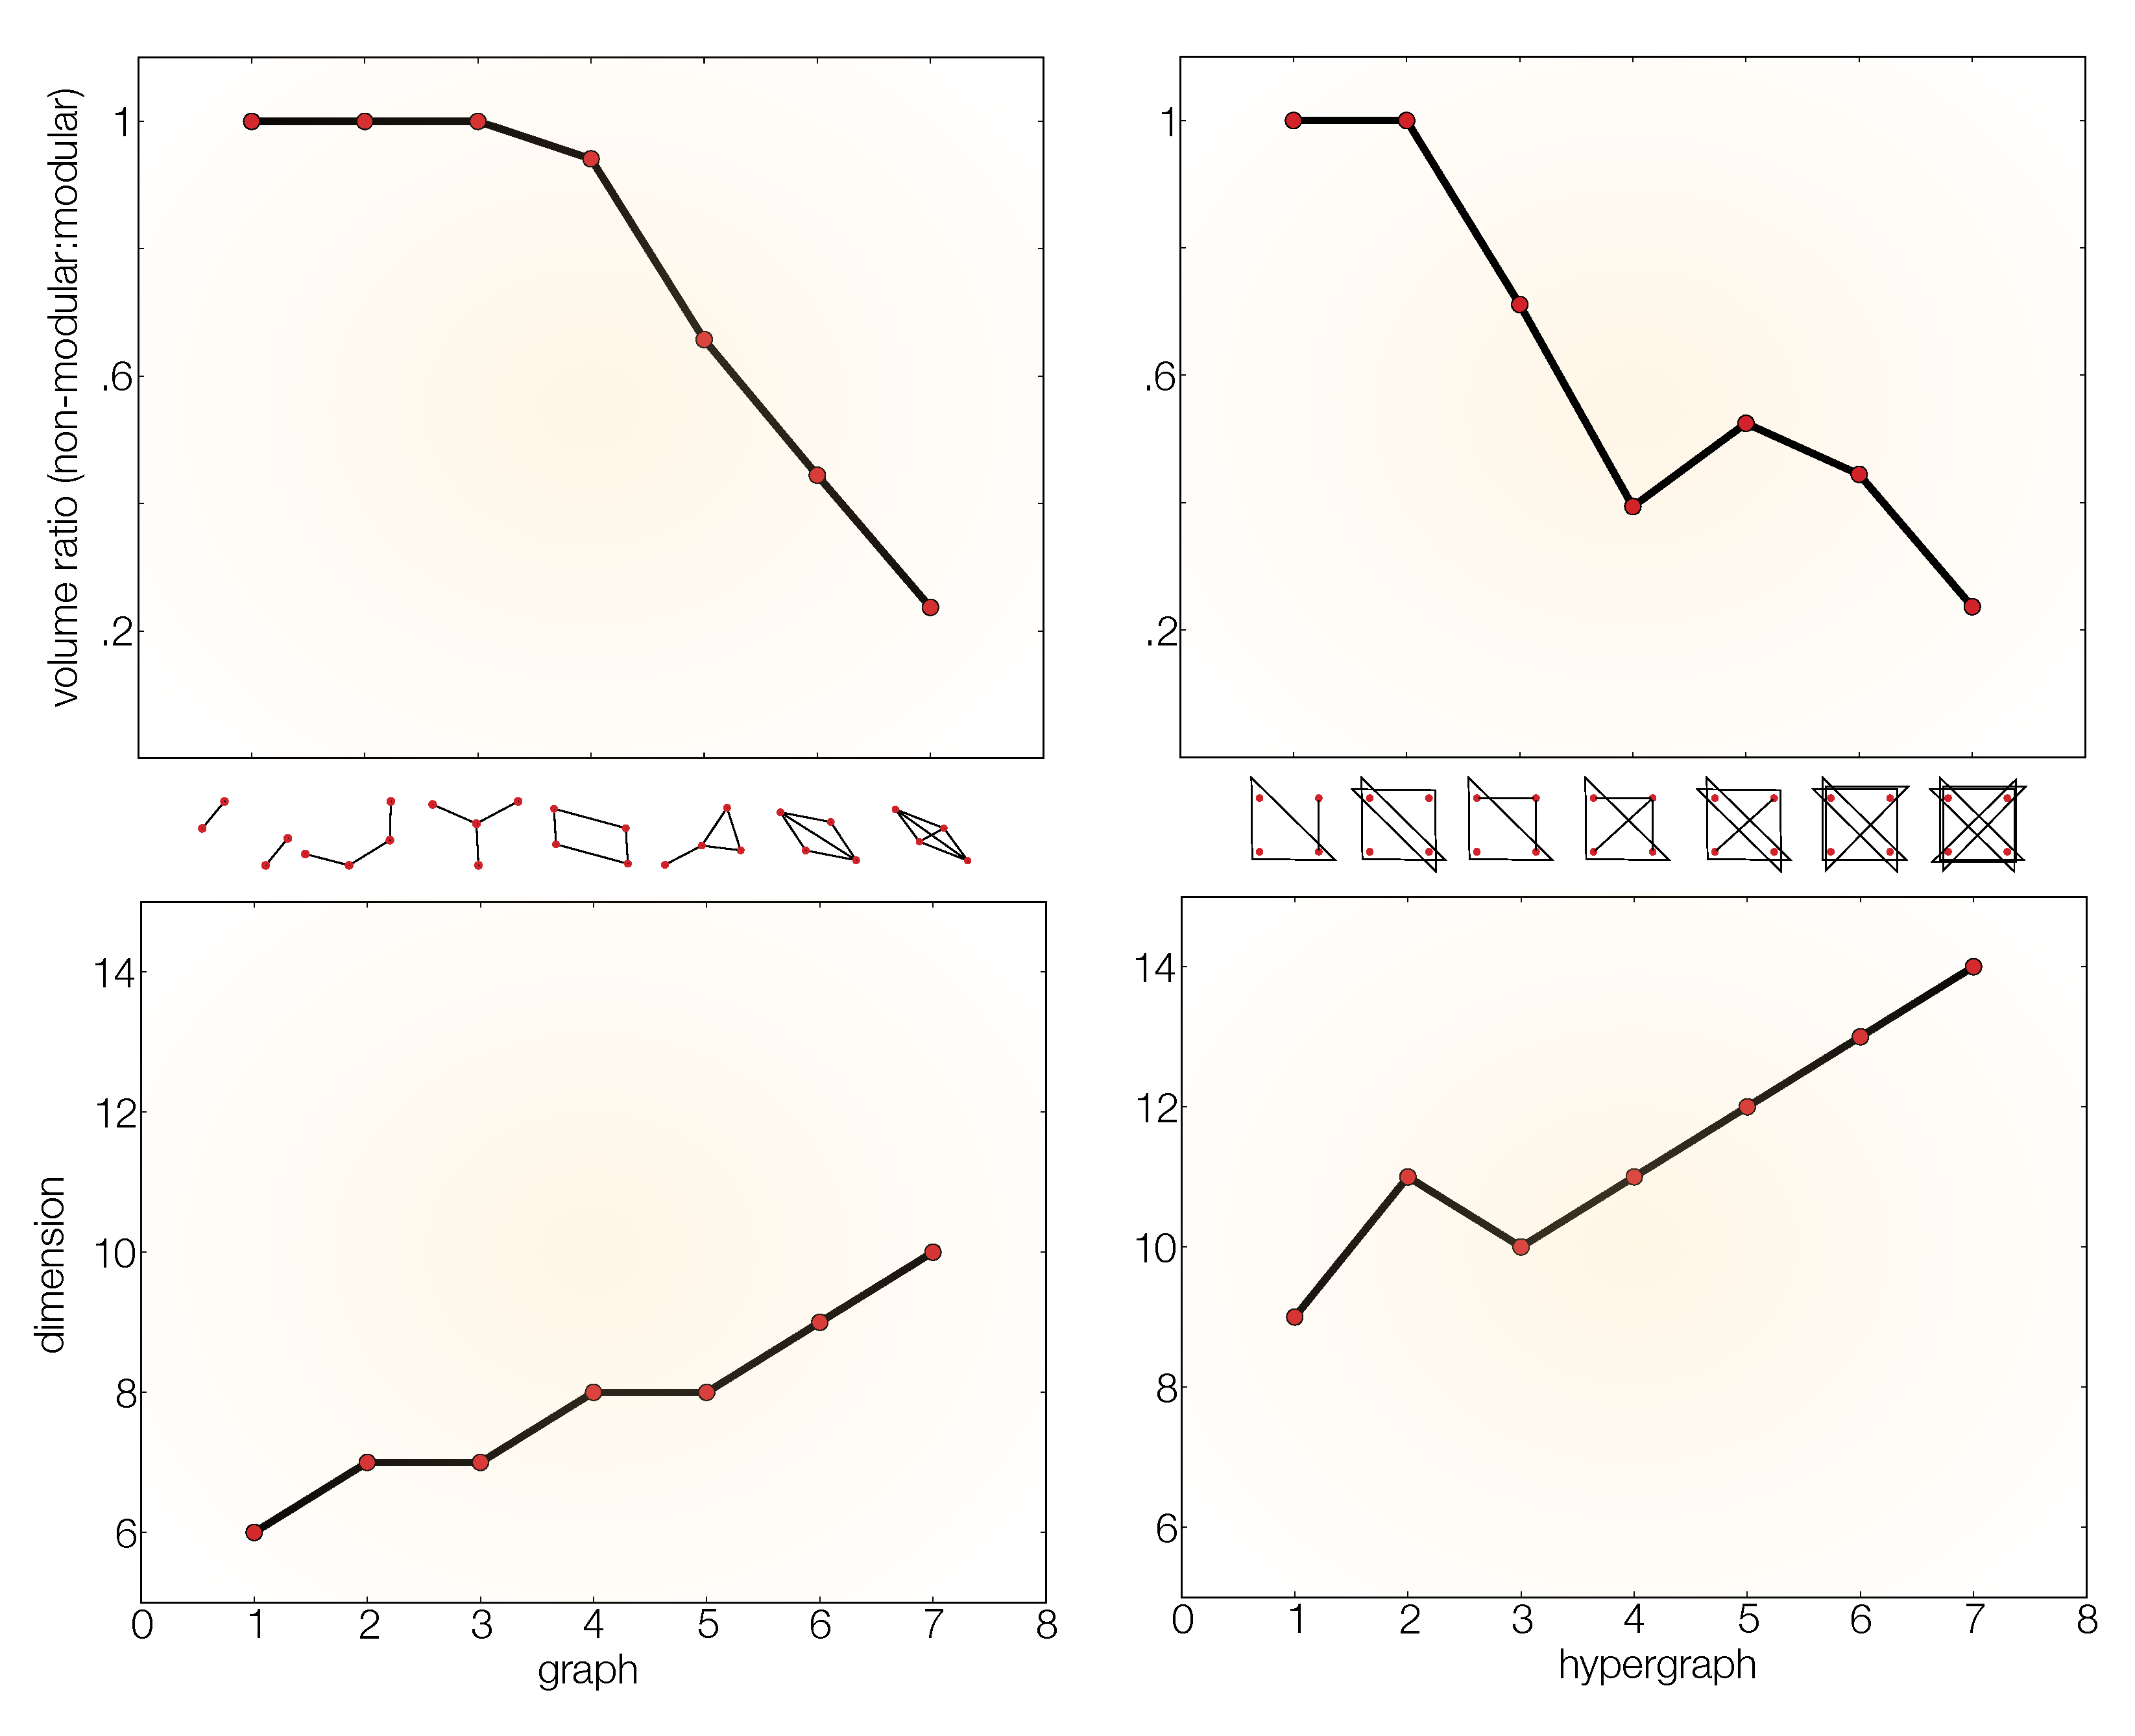
\includegraphics[width=0.9\columnwidth]{fig/figure_graphs_dims_nolines.pdf}
\caption{{\bf Non-modular to modular probability space volume ratio.} (A) and (B) show the ratio $\frac{\text{Vol}(\mathbb{M}(\mathcal{G}))}{\text{Vol}(\mathbb{L}(\mathcal{G}))}$ associated to 2-regular and non-2-regular GRNAs respectively. The (hyper)graph associated to each value of the volume ratio is displayed along the x-axis of each panel. (C) and (D) show the natural dimension of the space of probability distributions associated to $\mathbb{M}(\mathcal{G})$ and $\mathbb{L}(\mathcal{G})$ for each hypergraph.}
\label{fig:ncycvolrat}
\end{figure}

\begin{figure}[!ht]
\centering
\noindent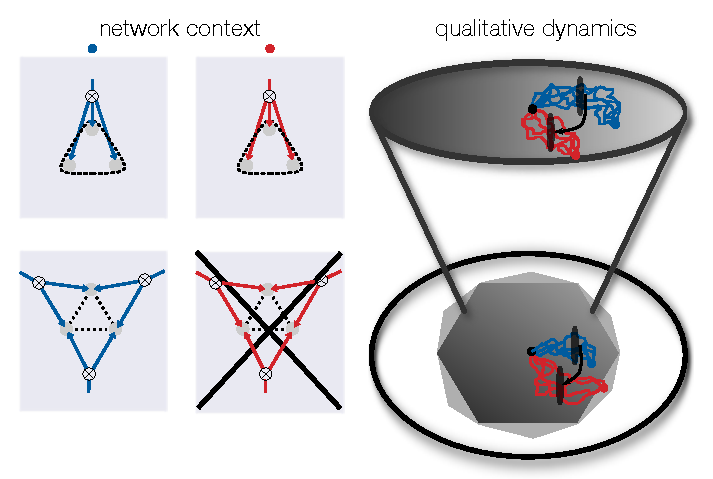
\includegraphics[width=0.9\columnwidth]{fig/stochdynscheme.pdf}
\caption{{\bf Schematic representation of the constraints imposed on stochastic gene expression and evolutionary dynamics by network architecture .} Schematic representation of a potential network context (left) for each of the hypothetical stationary probability distributions associated to the fitness peak established by the blue and red dots within the spaces of probability distributions represented on the right. Either of the two GRNAs represented on the left are capable of achieving the stationary distribution over genotype-phenotype mappings specified by the blue stationary distribution associated to a hypothetical fitness peak. On the other hand, only the GRNA from the top (and not the bottom) is capable of achieving the red stationary distribution representing an alternative potential fitness peak.}
\label{fig:stochdynscheme}
\end{figure}


\FloatBarrier

%\section{Tables}
%input{tex/table_hidvarmod}
%\begin{table}
\centering
\begin{subtable}[t]{0.4\textwidth}
\centering
\begin{tabular}{ l || c | c | c | r }
	$L_1 L_2$  &	00 & 01 & 10 & 11\\ \hline
    $l_1 l_2$ & $e_1$ & $e_2$ & $e_3$ & $e_4$\\ \hline
    $l_1 l'_2$ & $e_5$ & $e_6$ & $e_7$ & $e_8$\\ \hline
    $l'_1 l_2$ & $e_9$ & $e_{10}$ & $e_{11}$ & $e_{12}$\\ \hline
    $l'_1 l'_2$ & $e_{13}$ & $e_{14}$ & $e_{15}$ & $e_{16}$\\
    \hline
    \end{tabular}
    \caption{genotype-phenotype maps}
    \label{tab:gpm}
\end{subtable}
~~~~~~
\begin{subtable}[t]{0.4\textwidth}
\centering
	\begin{tabular}{ l || c | c | c | r }
	$L_1 L_2$  &	00 & 01 & 10 & 11\\ \hline
    $l_1 l_2$ & $p_1$ & $p_2$ & $p_3$ & $p_4$\\ \hline
    $l_1 l'_2$ & $p_5$ & $p_6$ & $p_7$ & $p_8$\\ \hline
    $l'_1 l_2$ & $p_9$ & $p_{10}$ & $p_{11}$ & $p_{12}$\\ \hline
    $l'_1 l'_2$ & $p_{13}$ & $p_{14}$ & $p_{15}$ & $p_{16}$\\
    \hline
	\end{tabular}
	\caption{probabilities}
    \label{tab:probabilities}
\end{subtable}
\caption{Genotype-phenotype mapping and associated probability tables for the two locus-two phenotype value example. We use an abbreviated notation in which we use the rewrite rules $l_1 l_2 \rightarrow \{l_1, l_2\}$ and $00 \rightarrow \{0, 0\}$ and all others analogous to avoid an excessive number of brackets.}
\label{tab:example}
\end{table}
%\begin{table}[!ht]
\centering
%!TEX root = ../plos_template.tex
\begin{subtable}[t]{0.4\textwidth}
\centering
\begin{tabular}{ l || c | r }
	$L$  &	0 & 1\\ \hline
    $l_1$ & \cellcolor{DeepBlue!35} $p^*_1$ & \cellcolor{DeepRed!35} $p^*_2$\\ \hline
    $l'_1$ & $p^*_3$ & $p^*_4$\\ \hline
    $l_2$ & $p^*_5$ & $p^*_{6}$\\ \hline
    $l'_2$ & $p^*_{7}$ & $p^*_{8}$\\
    \hline
    \end{tabular}
    \caption{$l_1$}
    \label{tab:il1}
\end{subtable}
~~~~~~
\begin{subtable}[t]{0.4\textwidth}
\centering
	\begin{tabular}{ l || c | c | c | r }
	$L_1 L_2$  &	00 & 10 & 01 & 11\\ \hline
    $l_1 l_2$ & \cellcolor{DeepBlue!35} $p_1$ & \cellcolor{DeepRed!35} $p_2$ & \cellcolor{DeepBlue!35} $p_3$ & \cellcolor{DeepRed!35} $p_4$\\ \hline
    $l_1 l'_2$ & \cellcolor{DeepBlue!35} $p_5$ & \cellcolor{DeepRed!35} $p_6$ & \cellcolor{DeepBlue!35} $p_7$ & \cellcolor{DeepRed!35} $p_8$\\ \hline
    $l'_1 l_2$ & $p_9$ & $p_{10}$ & $p_{11}$ & $p_{12}$\\ \hline
    $l'_1 l'_2$ & $p_{13}$ & $p_{14}$ & $p_{15}$ & $p_{16}$\\
    \hline
	\end{tabular}
	\caption{$l_1$}
    \label{tab:dl1}
\end{subtable}

\begin{subtable}[t]{0.4\textwidth}
\centering
\begin{tabular}{ l || c | r }
	$L$  &	0 & 1\\ \hline
    $l_1$ & $p^*_1$ & $p^*_2$\\ \hline
    $l'_1$ & \cellcolor{blue!25} $p^*_3$ & \cellcolor{green!25} $p^*_4$\\ \hline
    $l_2$ & $p^*_5$ & $p^*_{6}$\\ \hline
    $l'_2$ & $p^*_{7}$ & $p^*_{8}$\\    
    \hline
    \end{tabular}
    \caption{$l_2$}
    \label{tab:il2}
\end{subtable}
~~~~~~
\begin{subtable}[t]{0.4\textwidth}
\centering
	\begin{tabular}{ l || c | c | c | r }
	$L_1 L_2$  &	00 & 01 & 10 & 11\\ \hline
    $l_1 l_2$ & $p_1$ & $p_2$ & $p_3$ & $p_4$\\ \hline
    $l_1 l'_2$ & $p_5$ & $p_6$ & $p_7$ & $p_8$\\ \hline
    $l'_1 l_2$ & \cellcolor{blue!25} $p_9$ & \cellcolor{blue!25} $p_{10}$ & \cellcolor{green!25} $p_{11}$ & \cellcolor{green!25} $p_{12}$\\ \hline
    $l'_1 l'_2$ & \cellcolor{blue!25} $p_{13}$ & \cellcolor{blue!25} $p_{14}$ & \cellcolor{green!25} $p_{15}$ & \cellcolor{green!25} $p_{16}$\\
    \hline
	\end{tabular}
	\caption{$l_2$}
    \label{tab:dl2}
\end{subtable}
%!TEX root = ../plos_template.tex
\begin{subtable}[t]{0.4\textwidth}
\centering
\begin{tabular}{ l || c | r }
	$L$  &	0 & 1\\ \hline
    $l_1$ & $p^*_1$ & $p^*_2$\\ \hline
    $l'_1$ & $p^*_3$ & $p^*_4$\\ \hline
    $l_2$ & \cellcolor{DeepBlue!35} $p^*_5$ & \cellcolor{DeepRed!35} $p^*_{6}$\\ \hline
    $l'_2$ & $p^*_{7}$ & $p^*_{8}$\\
    \hline
    \end{tabular}
    \caption{$l_3$}
    \label{tab:il3}
\end{subtable}
~~~~~~
\begin{subtable}[t]{0.4\textwidth}
\centering
	\begin{tabular}{ l || c | c | c | r }
	$L_1 L_2$  &	00 & 10 & 01 & 11\\ \hline
    $l_1 l_2$ & \cellcolor{DeepBlue!35} $p_1$ & \cellcolor{DeepBlue!35} $p_2$ & \cellcolor{DeepRed!35} $p_3$ & \cellcolor{DeepRed!35} $p_4$\\ \hline
    $l_1 l'_2$ &  $p_5$ & $p_6$ & $p_7$ & $p_8$\\ \hline
    $l'_1 l_2$ & \cellcolor{DeepBlue!35} $p_9$ & \cellcolor{DeepBlue!35} $p_{10}$ & \cellcolor{DeepRed!35} $p_{11}$ & \cellcolor{DeepRed!35} $p_{12}$\\ \hline
    $l'_1 l'_2$ & $p_{13}$ & $p_{14}$ & $p_{15}$ & $p_{16}$\\
    \hline
	\end{tabular}
	\caption{$l_3$}
    \label{tab:dl3}
\end{subtable}

%!TEX root = ../plos_template.tex
\begin{subtable}[t]{0.4\textwidth}
\centering
\begin{tabular}{ l || c | r }
	$L$  &	0 & 1\\ \hline
    $l_1$ & $p^*_1$ & $p^*_2$\\ \hline
    $l'_1$ & $p^*_3$ & $p^*_4$\\ \hline
    $l_2$ & $p^*_5$ & $p^*_{6}$\\ \hline
    $l'_2$ & \cellcolor{DeepBlue!35} $p^*_{7}$ & \cellcolor{DeepRed!35} $p^*_{8}$\\
    \hline
    \end{tabular}
    \caption{$l_4$}
    \label{tab:il4}
\end{subtable}
~~~~~~
\begin{subtable}[t]{0.4\textwidth}
\centering
	\begin{tabular}{ l || c | c | c | r }
	$L_1 L_2$  &	00 & 10 & 01 & 11\\ \hline
    $l_1 l_2$ & $p_1$ & $p_2$ & $p_3$ & $p_4$\\ \hline
    $l_1 l'_2$ & \cellcolor{DeepBlue!35} $p_5$ & \cellcolor{DeepBlue!35} $p_6$ & \cellcolor{DeepRed!35} $p_7$ & \cellcolor{DeepRed!35} $p_8$\\ \hline
    $l'_1 l_2$ & $p_9$ & $p_{10}$ & $p_{11}$ & $p_{12}$\\ \hline
    $l'_1 l'_2$ & \cellcolor{DeepBlue!35} $p_{13}$ & \cellcolor{DeepBlue!35} $p_{14}$ & \cellcolor{DeepRed!35} $p_{15}$ & \cellcolor{DeepRed!35} $p_{16}$\\
    \hline
	\end{tabular}
	\caption{$l_4$}
    \label{tab:dl4}
\end{subtable}

\caption{The sheaf condition for the two-locus-two phenotype value example. The left column represents \emph{atomic} probabilities that relate probabilities via equations \ref{eq:pparsys} from the empirical models given in the right hand column. Each row in all tables is required to sum to 1.}
\label{tab:sheaf}
\end{table}

%\begin{table}[!ht]
\centering
\begin{tabular}{ c | l | c }
	\textbf{notation} & \textbf{description} & \textbf{size}\\ \hline \hline
	$\{l_1,l_2\}$ & set of genetic loci & $g = 2$\\ \hline
	$\{a_1,a_2\}$ & set of distinct alleles available to each locus & $a = 2$\\ \hline
	$\{0,1\}$ & set of phenotype values & $p = 2$\\ \hline
	$\{(0,0),(0,1),(1,0),(1,1)\}$ & set of phenotype assignments & $p^g = 4$\\ \hline
	$L = \{l_1,l_2,l'_1,l'_2\}$ & set of all possible alleles for all loci & $ga = 4$\\ \hline
	$\{l_1 l_2,l'_1 l_2,l_1 l'_2,l'_1 l'_2\}$ & set of gene regulatory network modules & $a^g = 4$\\ \hline
$\coprod_{O \in \mathcal{G}} \mathcal{E}(O)$ & set of modularized genotype-phenotype maps  & $(ap)^g = 16$\\ \hline
	$\mathcal{E}(L) = P^L$ & set of global genotype-phenotype maps & $p^{ga} = 16$\\
    \end{tabular}
\caption{Summary of concrete parameter values $(g,a,p)$ in terms of abstract notation for $(g=2,a=2,p=2)$. Note that $\{l_1,l_2,l'_1,l'_2\} \equiv \{l_1,l_2\} \times \{a_1,a_2\}$.}
\label{tab:pars222}
\end{table}

%%!TEX root = ../plos_template.tex
\begin{table}[!ht]
\centering
\begin{tabular}{ r || c | c | c | c | c | c | c | c | c | c | c | c | c | c | c | c }
		 &	\begin{sideways}$e^{1234}_{0000}$\end{sideways} & \begin{sideways}$e^{1234}_{0010}$\end{sideways} & \begin{sideways}$e^{1234}_{0001}$\end{sideways} & \begin{sideways}$e^{1234}_{0011}$\end{sideways}
			  & \begin{sideways}$e^{1234}_{1000}$\end{sideways} & \begin{sideways}$e^{1234}_{1010}$\end{sideways} & \begin{sideways}$e^{1234}_{1001}$\end{sideways} & \begin{sideways}$e^{1234}_{1011}$\end{sideways}
			  &	\begin{sideways}$e^{1234}_{0100}$\end{sideways} & \begin{sideways}$e^{1234}_{0110}$\end{sideways} & \begin{sideways}$e^{1234}_{0101}$\end{sideways} & \begin{sideways}$e^{1234}_{0111}$\end{sideways}
			  &	\begin{sideways}$e^{1234}_{1100}$\end{sideways} & \begin{sideways}$e^{1234}_{1110}$\end{sideways} & \begin{sideways}$e^{1234}_{1101}$\end{sideways} & \begin{sideways}$e^{1234}_{1111}$\end{sideways}\\ \hline \hline
    $e^{12}_{00}$ & 1 & 1 & 1 & 1 & 0 & 0 & 0 & 0 & 0 & 0 & 0 & 0 & 0 & 0 & 0 & 0\\ \hline
    $e^{12}_{10}$ & 0 & 0 & 0 & 0 & 1 & 1 & 1 & 1 & 0 & 0 & 0 & 0 & 0 & 0 & 0 & 0\\ \hline
    $e^{12}_{01}$ & 0 & 0 & 0 & 0 & 0 & 0 & 0 & 0 & 1 & 1 & 1 & 1 &  0 & 0 & 0 & 0\\ \hline
    $e^{12}_{11}$ & 0 & 0 & 0 & 0 & 0 & 0 & 0 & 0 & 0 & 0 & 0 & 0 & 1 & 1 & 1 & 1\\ \hline

    $e^{32}_{00}$ & 1 & 0 & 1 & 0 & 1 & 0 & 1 & 0 & 0 & 0 & 0 & 0 & 0 & 0 & 0 & 0\\ \hline
    $e^{32}_{10}$ & 0 & 1 & 0 & 1 & 0 & 1 & 0 & 1 & 0 & 0 & 0 & 0 & 0 & 0 & 0 & 0\\ \hline
    $e^{32}_{01}$ & 0 & 0 & 0 & 0 & 0 & 0 & 0 & 0 & 1 & 0 & 1 & 0 & 1 & 0 & 1 & 0\\ \hline
    $e^{32}_{11}$ & 0 & 0 & 0 & 0 & 0 & 0 & 0 & 0 & 0 & 1 & 0 & 1 & 0 & 1 & 0 & 1\\ \hline

    $e^{14}_{00}$ & 1 & 1 & 0 & 0 & 0 & 0 & 0 & 0 & 1 & 1 & 0 & 0 & 0 & 0 & 0 & 0\\ \hline
    $e^{14}_{10}$ & 0 & 0 & 0 & 0 & 1 & 1 & 0 & 0 & 0 & 0 & 0 & 0 & 1 & 1 & 0 & 0\\ \hline
    $e^{14}_{01}$ & 0 & 0 & 1 & 1 & 0 & 0 & 0 & 0 & 0 & 0 & 1 & 1 & 0 & 0 & 0 & 0\\ \hline
    $e^{14}_{11}$ & 0 & 0 & 0 & 0 & 0 & 0 & 1 & 1 & 0 & 0 & 0 & 0 & 0 & 0 & 1 & 1\\ \hline

    $e^{34}_{00}$ & 1 & 0 & 0 & 0 & 1 & 0 & 0 & 0 & 1 & 0 & 0 & 0 & 1 & 0 & 0 & 0\\ \hline
    $e^{34}_{10}$ & 0 & 1 & 0 & 0 & 0 & 1 & 0 & 0 & 0 & 1 & 0 & 0 & 0 & 1 & 0 & 0\\ \hline
    $e^{34}_{01}$ & 0 & 0 & 1 & 0 & 0 & 0 & 1 & 0 & 0 & 0 & 1 & 0 & 0 & 0 & 1 & 0\\ \hline
    $e^{34}_{11}$ & 0 & 0 & 0 & 1 & 0 & 0 & 0 & 1 & 0 & 0 & 0 & 1 & 0 & 0 & 0 & 1\\
    \end{tabular}
\caption{Explicit construction of $\mathbf{G}_{n \times m}$ for the case $L = \{ l_1,l_2,l_3,l_4 \}$, $\mathcal{G} = \{\{l_1,l_2 \},\{l_1,l_4 \},\{l_3,l_2\},\{l_3,l_4\} \}$, $P=\{0,1\}$ and thus $\mathbf{G}_{(2 \cdot 2)^2 \times 2^{2 \cdot 2}} = \mathbf{G}_{16 \times 16}$.}
\label{tab:logmat222}
\end{table}


%\FloatBarrier

\pagebreak
\setcounter{secnumdepth}{4}
\section{Supplementary Material}
%!TEX root = ../plos_template.tex
\subsection{Deterministic genotype-phenotype maps}
Consider the case in which we have an arbitrary number of \emph{genes} indexed by $i=1, \ldots, m$. There is a particular set of potential \emph{genes} denoted $L$. A subset of genes will be denoted as $U \subseteq L$. We also have a set of phenotypes $P$. In principle, any gene could give rise to any phenotype. A genotype-phenotype map is thus represented as a function mapping a subset of genes into phenotypes
$$
e \colon U \rightarrow  P.
$$

In the operationalist framework from which this modeling description derives \cite{Abramsky2011}, our genes and subsets thereof $U \subseteq L$ are analogous to measurements and subsets thereof $T \subseteq X$ and our phenotypes $P$ are like measurement outcomes or values $V$. An event in which outcomes $s(t)$ are observed for each $t \in T$ serve to define mappings called \emph{sections} over $T$ as

$$
s \colon T \rightarrow V.
$$

We denote the set of all subsets of a set $X$ as $\mathcal{P}(X)$. $\mathcal{P}(L)$ can then be viewed as a category~\cite{Lane1998,MacLane1992,Awodey2006} in which the objects are subsets of genes and morphisms represent inclusion of a smaller subset into a larger superset (i.e. $U \subseteq U' \Rightarrow U \rightarrow U'$). The category $\mathcal{P}(L)^{opp}$ then has the same objects, but the morphisms represent restriction from a larger to a smaller subset of genes (i.e. $U' \supseteq U \Rightarrow U' \rightarrow U$). In order to consider the set of all genotype-phenotype maps, for a given set of genes $L$, together, we can construct a functor
$$
\mathcal{E} \colon \mathcal{P}(L)^{opp} \rightarrow Set
$$
by exhibiting precisely how it acts on objects and morphisms in its domain category. We explicitly represent the way in which the functor $\mathcal{E}$ acts on objects $U$ and morphisms $U \subseteq U'$ respectively as
\begin{equation}\label{eq:gpfunctor}
\begin{split}
\mathcal{E} \colon \mathcal{P}(L)^{opp} &\rightarrow Set,\\
U &\mapsto P^U,\\
U \subseteq U' &\mapsto res^{U'}_{U}.
\end{split}
\end{equation}
So the functor $\mathcal{E}$ takes a subset of genes and returns the set of genotype-phenotype mappings from the given subset of genes to the set of phenotypes. The restriction map operates on sets deriving from the application of $\mathcal{E}$ to a subset of genes as follows
\begin{eqnarray*}
res^{U'}_{U} \colon \mathcal{E}(U') &\rightarrow& \mathcal{E}(U)\\
P^{U'} &\rightarrow& P^U\\
e' \colon U' \rightarrow P &\mapsto& e'|_U \colon U \rightarrow P
\end{eqnarray*}
$\mathcal{E}$ is thus, by definition, a presheaf functor, which is an object in the functor category $Sets^{\mathcal{P}(L)^{opp}}$.

\subsection{Stochasticity among genotype-phenotype maps}
There may be several sources for stochasticity in genotype-phenotype mapping including small numbers of the causal molecules and products of gene expression as well as environmental fluctuations upon which genotype-phenotype mappings are conditioned \cite{Swain2002,Paulsson2004,Thattai2004,Acar2008a,Lestas2010,Munsky2012,Chalancon2012,Neuert2013,Sanchez2013}. Regardless of the fundamental nature of stochasticity to gene expression, empirically, we observe statistical as opposed to deterministic data. Here we generalize the deterministic framework outlined above to the stochastic case.

An \emph{algebraic structure} is determined by a set and one or more finitary operations (e.g. binary multiplication) defined on the elements of that set \cite{PachterLior2005,Artin2010}. A \emph{monoid} is a type of algebraic structure determined by a set and a binary operation such that the latter satisfies closure, associativity and identity with respect to the given set. A \emph{semiring} is an algebraic structure determined by a set with two binary operations. One of the binary operations, addition, forms a commutative monoid and has identity element 0. The second binary operation, multiplication, is a monoid with identity element 1. These binary operations interact such that multiplication distributes over addition and multiplication by the identity element of the addition monoid annihilates all elements in the semiring. For example, the real numbers under addition and multiplication constitute a semiring whose data is described as $\left( \mathbb{R},+,0,\times,1 \right)$.

Consider a function, $\phi$ from a set, $L$, to a semiring $R$ written $\phi \colon L \rightarrow R$. The \emph{support} of $\phi$, $\text{supp}(\phi)$, is then the set $\{ l \in L | \phi(l) \neq 0 \}$. A distribution with respect to the semiring $R$ on $L$ is given as a function having finite support and satisfying a constraint
\begin{eqnarray*}
d \colon L \rightarrow R,\\
\sum_{l \in L} d(l) = 1
\end{eqnarray*}
We can consider the set of all distributions with respect to a given semiring $R$ satisfying the above constraints and defined on the set $L$ as being given by a functor applied to $L$ as $\mathcal{D}_R (L)$. We can again explicitly represent the way in which the functor $\mathcal{D}_R$ acts on objects and morphisms $L$ and $f \colon L \rightarrow M$ (where $L$ and $M$ are sets viewed as sets of genes and in some special cases we may have $M=L$) as
\begin{equation}\label{eq:distfunctor}
\begin{split}
\mathcal{D}_R \colon Set &\rightarrow Set,\\
L &\mapsto \mathcal{D}_R (L),\\
f \colon L \rightarrow M &\mapsto \mathcal{D}_R (f) \colon \mathcal{D}_R (L) \rightarrow \mathcal{D}_R (M),
\end{split}
\end{equation}
where
\begin{eqnarray*}
\mathcal{D}_R (f) \colon \mathcal{D}_R (L) &\rightarrow& \mathcal{D}_R (M),\\
d &\mapsto& \left[ m \mapsto \sum_{f(l)=m} d(l) \right].
\end{eqnarray*}
For the case in which we consider $R$ to be the semiring of non-negative real numbers $\left( \mathbb{R}_{\geq 0},+,0,\times,1 \right)$, $\mathcal{D}_R (L)$ represents the set of probability distributions over the set $L$.

Recalling the presheaf functor, $\mathcal{E} \colon \mathcal{P}(L)^{opp} \rightarrow Set$, mapping genotypes to the set of maps from those genotypes to the set of phenotypes, we can now compose it with the distribution functor $\mathcal{D}_R$ to obtain a new presheaf functor $\mathcal{D}_R \circ \mathcal{E} \colon \mathcal{P}(L)^{opp} \rightarrow Set \rightarrow Set$ that assigns to each genotype a distribution over the set of maps from those genotypes to the set of possible phenotypes. The action of $\mathcal{D}_R \mathcal{E}$ on objects and morphisms in $\mathcal{P}(L)^{opp}$ yields
\begin{eqnarray*}
\mathcal{D}_R \mathcal{E} \colon \mathcal{P}(L)^{opp} &\rightarrow& Set,\\
U &\mapsto& \mathcal{D}_R \mathcal{E}(U) \equiv d \colon P^U \rightarrow R,\\
U \subseteq U' &\mapsto& \mathcal{D}_R \mathcal{E}(U') \rightarrow \mathcal{D}_R \mathcal{E}(U).
\end{eqnarray*}
where
\begin{eqnarray*}
\mathcal{D}_R \mathcal{E}(U') &\rightarrow& \mathcal{D}_R \mathcal{E}(U),\\
d \colon P^{U'} \rightarrow R &\rightarrow& d|U \colon P^{U} \rightarrow R
\end{eqnarray*}
and
\begin{eqnarray*}
d \colon P^{U'} &\rightarrow& R,\\
s' &\mapsto& d(s');\\
d|U \colon P^{U} &\rightarrow& R,\\
s &\mapsto& \sum_{s' \in \mathcal{E}(U'),\, s'|U=s} d(s').
\end{eqnarray*}
$d|U$ is a representation of what is commonly referred to as the marginal distribution of $d$ that assigns to each genotype-phenotype mapping in the smaller collection (recall $U \subseteq U'$) of such $P^{U}$ the sum of the probabilities of all genotype-phenotype maps in the larger collection $P^{U'}$ that restrict to a given map in $P^{U}$.

\subsection{Coverings of genotype space}
A \emph{gene regulatory network module} is represented by a subset of genes $O$ and a collection of gene regulatory network modules, which in some cases may represent all of the genes in an organism, is a set of such subsets $\mathcal{G}$ (i.e. $O,O',\ldots \in \mathcal{G}$). An individual may be composed of some collection of subsets of possible genes where the set of all genes, $L$, is viewed as the genotype space. A \emph{covering} of the genotype space, $\mathcal{G}$, satisfies 1. $\cup_i O_i = \cup \mathcal{G} = L$ and 2. if $O,O' \in \mathcal{G}$ and $O \subseteq O'$ means that $O = O'$. The first condition means that $\mathcal{G}$ covers $L$. It is thereby just a statement that $\mathcal{G}$ represents a decomposition of the collection of all genes under consideration into subsets and this is why we refer to $\mathcal{G}$ as a collection of gene regulatory network modules. The second condition means simply that we will not consider nested subsets and so we will take for our $O \in \mathcal{G}$ the biggest $O \in \mathcal{G}$ that is not a subset of some other $O' \in \mathcal{G}$. The second condition also implies that if a given subset of genes $O'$ is compatible in a sense to be explained more precisely in what proceeds then any smaller subset of genes $O$ is also compatible. Coverings $\mathcal{G}$ of the genotype space contain the necessary information to make precise what we heuristically refer to at other points in this paper as modularity in order to cohere with standard terminology in systems biology literature while attempting to submit our own precise interpretation of the relatively colloquial concept.

\subsection{Compatibility of distributions on genotype-phenotype maps}
Given a covering of the genotype space $\mathcal{G}$, a compatible family for $\mathcal{G}$ with respect to the distribution presheaf $\mathcal{D}_R\mathcal{E}$ is given by a family of distributions $\{d_O \colon P^O \rightarrow R | O \in \mathcal{G}\}$ such that for all $O \in \mathcal{G}$ there exists $d_O \in \mathcal{D}_R\mathcal{E}(O)$ such that for all $O' \in \mathcal{G}$
\begin{eqnarray}\label{eq:sheafcond}
%\forall O \in \mathcal{G} \left[ \exists d_O \in \mathcal{D}_R\mathcal{E}(O) \right],\\
d_O|O \cap O' = d_{O'}|O \cap O'.
\end{eqnarray}
The condition \ref{eq:sheafcond} is referred to as the \emph{sheaf condition}. This condition means that any two distributions $d_O$ and $d_{O'}$ in the \emph{compatible family} of distributions produce the same values in the semiring $R$ on all of the genes in the intersection of $O$ with $O'$.

For example, if we have two gene regulatory network modules given by their genotypes $O = \{l_1, l_2\}$ and $O' = \{l_1, l_3\}$ then the sheaf condition specifies that for $e_{\{l_1\}} \in \mathcal{E}(\{l_1\})$, which assigns a particular phenotype to the genotype $\{l_1\}$ rather than to an entire gene regulatory network module like $O$ or $O'$, that
\begin{eqnarray}\label{eq:sheafprob}
\sum_{e \in \mathcal{E}(O),\, e|l_1=e_{\{l_1\}}} d_O(e) \,\, = \sum_{e' \in \mathcal{E}(O'),\, e'|l_1=e_{\{l_1\}}} d_{O'}(e')
\end{eqnarray}
This condition means that the probability for gene $l_1$ to be associated to the phenotype given by $e_{\{l_1\}}$ is equivalent in case we marginalize over all the other genes contained in the gene regulatory network modules of which $l_1$ is a component. For coherence with respect to the relationship between the modeling framework described here and that used in probabilistic graphical models in machine learning, the conditions \ref{eq:sheafprob} are referred to as the marginalization constraints \cite{Wainwright2007}.

\subsection{Global sections of distributions over genotype-phenotype maps}
To say that the sheaf condition holds for a compatible family $\{d_O\}_{O \in \mathcal{G}}$ for the presheaf $\mathcal{D}_R\mathcal{E}$ implies the existence of a \emph{global section} $d \in \mathcal{D}_R\mathcal{E}(L)$ that is defined on the full set of genes. An example of a distribution that could be a global section given that it satisfies the sheaf condition is shown in \ref{tab:hidvarmod}. This global section defines a distribution on the set of genotype-phenotype maps given by $\mathcal{E}(L) = P^L$, specifying phenotypes associated to all genes at once instead of on subsets of $L$ associated to either $U \subseteq L$ or, what is essentially equivalent, $O \in \mathcal{G}$. Crucially, the distribution $d$ must also restrict for the subset of genes associated to any gene regulatory network module, which in some cases may represent all of the genes in an organism, $O$ in a covering of the genotype space $\mathcal{G}$ meaning that
\begin{eqnarray}
\forall O \in \mathcal{G} \left[ d|O = d_O \right].
\end{eqnarray}
In terms of distributions, the existence of a global section $d$ for a covering of the genotype space $\mathcal{G}$ corresponds to the existence of a distribution defined on all genes that marginalizes to yield the distributions on subsets of genes that may be observed empirically.

The presheaf $\mathcal{E}$ alone was already a sheaf because given a cover $\{U_i\}_{i \in I}$ of $U$ there is a family of sections $\{e_i \in \mathcal{E}(U_i)\}_{i \in I}$ that is compatible in the sense that
\begin{eqnarray}
\forall i,j \in I \left[ e_i|U_i \cap U_j = e_j|U_i \cap U_j \right].
\end{eqnarray}
In this case there is a unique global section $e \in \mathcal{E}(U)$ such that $\forall i \in I \left[ e|U_i = e_i \right]$. The fact that the sheaf condition holds for $\mathcal{E}$ is true because we are considering functions defined on a space with a trivial discrete topology allowing us to combine any partial functions that agree on overlapping subsets by taking the union of the data defining such functions.

Extending this example on an arbitrary subset $U \subseteq L$ to the whole set of genes $L$ we have a unique global section $e \in \mathcal{E}(L) = P^L$. $e$ can be used to deterministically assign phenotypes to the set of genes $L$ under consideration.

\subsection{Example}
We can construct an example to make the model description, so far, more concrete. For this example, we take the full set of potential genes to be $L = \{ l_1,l_2,l_3,l_4 \}$. Consider the case in which each of the gene regulatory network modules under consideration has two genes and we specify the covering of the genotype space given by $\mathcal{G} = \{\{l_1,l_2 \},\{l_1,l_4 \},\{l_3,l_2\},\{l_3,l_4\} \}$. The full set of genes together with a covering of the genotype space is a special case of a hypergraph $\mathcal{H} = (L,\mathcal{G})$ where the set of genes $L$ serve as the nodes or vertices and the covering $\mathcal{G}$ contains the edges or hyperedges. We also have two phenotype values $P = \{0, 1\}$. Each genotype-phenotype map in \ref{tab:gpm} assigns phenotype values to each $O \in \mathcal{G}$. For example, $e_1 \colon   l_1 l_2 \rightarrow 00$. \ref{tab:probabilities} likewise assigns probabilities to each of these genotype-phenotype mappings.

We can collect all of these genotype-phenotype mappings into one set using the functor given in \ref{eq:gpfunctor} as $\mathcal{E}(\mathcal{G}) = P^{\mathcal{G}} = \{e_i | i=1 \ldots 16 \}$. We may further apply the $R$-distribution functor $\mathcal{D}_R$ given in \ref{eq:distfunctor} to obtain a distribution on the genotype-phenotype mappings. Doing so yields  $\mathcal{D}_R\mathcal{E}(\mathcal{G})=d \colon P^\mathcal{G} \rightarrow R$. If we now apply this distribution function $d$ to the set of genotype-phenotype mappings we get the probabilities associated to each genotype-phenotype map $d(\{e_i | i=1 \ldots 16 \}) = \{p_i|i=1 \ldots 16\}$ given in \ref{tab:probabilities}. This can also be written more abstractly as $\left[\mathcal{D}_R\mathcal{E}(\mathcal{G})\right](\{e_i | i=1 \ldots 16 \}) = \left[\mathcal{D}_R\mathcal{E}(\mathcal{G})\right](P^\mathcal{G}) = \left[\mathcal{D}_R\mathcal{E}(\mathcal{G})\right](\mathcal{E}(\mathcal{G})) = \{p_i|i=1 \ldots 16\}$. Notice that we applied the functors $\mathcal{E}$ and $\mathcal{D}_R$ to a specific set, which was all of $\mathcal{G}$. We could have applied these functors to any $O \in \mathcal{G}$. In one case, for example if we take $O = \{l_1, l_2\}$, we would have gotten $\mathcal{E}(O) = \{e_i|i=1 \ldots 4\}$ and $\mathcal{D}_R\mathcal{E}(O) = d \colon P^O \rightarrow R$. In this case $\left[\mathcal{D}_R\mathcal{E}(O)\right](\mathcal{E}(O)) = \{p_i|i=1 \ldots 4\}$.

We may also consider directly the meaning of $\left[\mathcal{D}_R\mathcal{E}(\{l_1\})\right](\mathcal{E}(\{l_1\}))$ and similarly for the other $l \in L$. The sheaf condition then introduces a system of equations relating and thus constraining the probability parameters, beyond the constraint that each row sum to one. The constraint introduced by the sheaf condition is expressed in \ref{eq:sheafprob}, specialized to this example by
\begin{eqnarray}\label{eq:sheafprob2}
\sum_{e \in \mathcal{E}(\{l\}),\, e|l=e_{\{l\}}} d_{\{l\}}(e) \,\, = \sum_{e \in \mathcal{E}(O),\, e|l=e_{\{l\}}} d_O(e) \,\, = \sum_{e' \in \mathcal{E}(O'),\, e'|l=e_{\{l\}}} d_{O'}(e'),
\end{eqnarray}
for each $l \in L$, $e_{\{l\}} \in \mathcal{E}(\{l\})$, and $\{O \in \mathcal{G}|l=o, o \in O\}$. The resulting equations are explicitly indicated in like colors between the columns of \ref{tab:sheaf} :
\begin{equation}
\begin{aligned}\label{eq:pparsys}
p^*_1 &= p_1 + p_3 = p_5 + p_7, &
p^*_2 &= p_2 + p_4 = p_6 + p_8,\\
p^*_3 &= p_9 + p_{11} = p_{13} + p_{15},&
p^*_4 &= p_{10} + p_{12} = p_{14} + p_{16},\\
p^*_5 &= p_1 + p_2 = p_9 + p_{10},&
p^*_6 &= p_3 + p_4 = p_{11} + p_{12},\\
p^*_7 &= p_5 + p_6 = p_{13} + p_{14},&
p^*_8 &= p_7 + p_8 = p_{15} + p_{16}.
\end{aligned}
\end{equation}

Consider the meaning of the sheaf condition for $\mathcal{D}_R\mathcal{E}(L)$. $d \in \mathcal{D}_R\mathcal{E}(L)$ specifies a distribution whose domain consists of deterministic functions $\mathcal{E}(L) = P^L$ that map each gene independently, and independent of the fact that some combinations of genes  comprise gene regulatory network modules consisting of potentially interacting genes, to a phenotype. Since we have stated that $\mathcal{E}(L)$ satisfies the sheaf condition, for a given covering of the genotype space, $\mathcal{G}$, a globally compatible function $e \in  \mathcal{E}(L)$ restricts to $e|O$ for each $O \in \mathcal{G}$ such that there is a tuple of phenotypes assigned to genes that participate in overlapping gene regulatory network modules. Each $e \in P^L$ is associated to a trivial distribution $\delta_e \in \mathcal{D}_R\mathcal{E}(L)$ such that
\begin{eqnarray}
\delta_e(e') =
\begin{cases}
1, & e' = e,\\
0, & e' \neq e.
\end{cases}
\end{eqnarray}
For each gene regulatory network module $O$ we note that $\delta_e|O = \delta_{e|O}$. In this case, we can write the empirically determined distribution such as \ref{tab:probabilities} for a particular gene regulatory network module $d_O$ in terms of the distribution defined on the global set of genes restricted to a particular gene regulatory network module $d|O$:
\begin{equation}\label{eq:factordist}
\begin{split}
d_O(e) &= d|O(e)\\
&= \sum_{e' \in \mathcal{E}(L),e'|O=e} d(e')\\
&= \sum_{e' \in \mathcal{E}(L)} \delta_{e'|O}(e) \, d(e') = \sum_{e' \in \mathcal{E}(L)} \delta_{e'}|O(e) \, d(e')
\end{split}
\end{equation}
where
\begin{equation*}
\delta_{e'}|O(e) = \prod_{o \in O} \delta_{e'|\{o\}}(e|\{o\}).
\end{equation*}
We recover the empirically determined distribution as a sum over the deterministic genotype-phenotype mappings weighted by the probabilities of the distribution $d \in \mathcal{D}_R\mathcal{E}(L)$ defined over the full set of such deterministic mappings.

Thus, when there is a global section, given by $d \in \mathcal{D}_R\mathcal{E}(L)$, for an empirically determined distribution on genotype-phenotype mappings, for example that in \ref{tab:probabilities}, then it may be the case that a mechanism that stochastically selects among deterministic genotype-phenotype maps can satisfy or generate an empirically determined distribution.

\subsection{Existence of a global section for an empirically determined distribution of genotype-phenotype mappings}
Given an empirically determined distribution on the genotype-phenotype mapping process, it may be helpful to be able to classify whether or not there exists a global section satisfying the sheaf condition in order to determine the modularity requirements of the empirical distribution. If an empirically determined distribution does have a global section, then it is possible to achieve the same global biological function specified in the empirical distribution using a single gene regulatory network module that contains all of the genes in the given universal set of genes $L$ as is obtained using the particular cover of the genotype space $\mathcal{G}$ that is associated to the empirically determined distribution. If the empirically determined distribution does not have a global section satisfying the sheaf condition, then there is some contingency regarding interactions between genes necessitating decomposition into smaller submodules than is represented by the whole of the universal set of genes $L$.

For a cover of the genotype space, $\mathcal{G}$, we can construct an incidence matrix, $\mathbf{G}$, representing the relationship between genotype-phenotype mappings having as domain particular gene regulatory network module contexts given by the $O \in \mathcal{G}$ and those global genotype-phenotype mappings defined on $L$. This is equivalent to the more formal statement that there is some binary relation,
\begin{equation}
R \subseteq \mathcal{E}(L) \times \coprod_{O \in \mathcal{G}} \mathcal{E}(O),
\end{equation}
whose \href{http://en.wikipedia.org/wiki/Logical_matrix#Matrix_representation_of_a_relation}{logical matrix representation}, $\mathbf{G}$, we would like to construct. In the first case, $\mathcal{E}(L) = P^L$ we have $\{t_1, \ldots t_m\} = \{t_j | t_j \in P^L\}$. In the second case, $\coprod_{O \in \mathcal{G}} \mathcal{E}(O)$, we have $\{e_1, \ldots e_n\} = \coprod_{O \in \mathcal{G}} \mathcal{E}(O)$. So we have two sets of maps, one defined on $P^L$ and the other defined on $\mathcal{E}(O) = P^O$ for each $O \in \mathcal{G}$. This yields a method of specifying the intended relationship that defines $\mathbf{G}_{n \times m}$ in terms of $t_j \in P^L$ and $e_i \in \mathcal{E}(O)$ :
\begin{eqnarray}
\mathbf{G}[i,j] =
\begin{cases}
1, & t_j|O = e_i,\\
0, & \text{otherwise}.
\end{cases}
\end{eqnarray}
This matrix can be viewed as an operator acting via matrix multiplication on distributions
\begin{eqnarray*}
\mathbf{G} \colon \mathcal{D}_R\mathcal{E}(L) &\rightarrow& \mathcal{D}_R\mathcal{E}(\mathcal{G}),\\
d &\mapsto& (d|O)_{O \in \mathcal{G}},
\end{eqnarray*}
and thereby taking a global distribution defined on genotype-phenotype maps whose domain is the full set of genes $L$ to the \emph{marginalized} distributions that are defined relative to gene regulatory network modules contained in a covering of the genotype space $\mathcal{G}$. This is to say that $\mathbf{G} \cdot d = (d|O)_{O \in \mathcal{G}} = \{d_O\}_{O \in \mathcal{G}}$. $\mathbf{G}$ provides a way of determining the kinds of environmentally determined distributions on genotype-phenotype mapping (i.e. $\{d_O\}_{O \in \mathcal{G}}$, \ref{tab:probabilities}) that can be derived from distributions (i.e. $\mathcal{D}_R \mathcal{E}(L)$) defined on the global genotype-phenotype mappings (i.e. $\mathcal{E}(L)$ as opposed to $\mathcal{E}(O)$).

If we have an experimentally determined distribution on genotype phenotype maps in different genetic contexts (e.g. in \ref{tab:probabilities}) that we refer to as $\{d_O\}_{O \in \mathcal{G}}$, then we have an assignment of a probability value in $R$ to each genotype phenotype map $e_i \in \mathcal{E}(O)$ in \ref{tab:gpm}. We can collect these probabilities into a vector $\mathbf{V}_{n \times 1}$ where we note that $n$ is the same as that used to specify the number of genotype-phenotype maps in the coproduct over gene regulatory network modules in a given covering of the genotype space $\{e_1, \ldots e_n\} = \coprod_{O \in \mathcal{G}} \mathcal{E}(O)$. We can specify as unknown a distribution on the set of globally defined genotype phenotype maps and collect the associated probabilities in a vector $\mathbf{X}_{m \times 1}$ where there is a probability weight associated to each $t_j \in \mathcal{E}(L)$. Now we can attempt to determine the probability distribution on globally defined genotype-phenotype mappings $\mathcal{E}(L)$ by solving the linear system of equations
\begin{equation}
\begin{split}
\mathbf{G}_{n \times m} \mathbf{X}_{m \times 1} = \mathbf{V}_{n \times 1},\\
\sum_{i=1}^{m} \mathbf{X}_{i} = 1.
\end{split}
\end{equation}
The constraint that $\mathbf{X}$ sum to one in order to satisfy the definition of a probability distribution can be integrated into the matrix equation by adjoining a row containing ones to $\mathbf{G}_{n \times m}$ and a row containing a one to $\mathbf{V}_{n \times 1}$
\begin{equation}\label{eq:auglinsys}
\mathbf{G}_{(n + 1) \times m} \mathbf{X}_{m \times 1} = \mathbf{V}_{(n + 1) \times 1}.
\end{equation}
Solutions, if any, to \ref{eq:auglinsys} serve to exhibit a global section for the empirically determined distribution specified in $\mathbf{V}$.

% \subsection{Example global section determination}
% There are three parameters that determine the relative size of important sets for understanding the model at hand. $g$ represents the number of genetic loci, $a$ represents the number of different alleles that can occur at each locus, and $p$ represents the number of different phenotype values that each locus can take on. From these parameters, which we use together to classify models satisfying the structural constraints described thus far, we can derive additional quantities characterizing the model. For a system with parameters $(g,a,p)$ there are $a^g$ different gene regulatory network modules to consider and each may be associated with $p^g$ phenotypes. There are thus $(ap)^g$ different genotype-phenotype maps to consider with respect to the gene regulatory network modules meaning that this is the size of the set $\coprod_{O \in \mathcal{G}} \mathcal{E}(O)$. The set of all possible genes $L$ has size $ga$ and since there are $p$ different phenotypes that each gene can be mapped to, there are $p^{ga}$ different globally defined genotype-phenotype maps meaning that this is the size of the set $\mathcal{E}(L) = P^L$. Now we can state the size of the sets $\{t_1, \ldots t_m\} = \{t_j | t_j \in P^L\}$ and $\{e_1, \ldots e_n\} = \coprod_{O \in \mathcal{G}} \mathcal{E}(O)$ because we have explicit formulas for $n = (ap)^g$ and $m = p^{ga}$ in terms of the defining characteristics of a $(g,a,p)$ class of models. From the values of $n$ and $m$ we know the dimensions of the logical matrix representation of the relation $R$ as $\mathbf{G}_{(ap)^g \times p^{ga}}$.

% For the case $(g=2,a=2,p=2)$, \ref{tab:pars222} shows the relationship between the abstract notation used throughout the model description and the concrete parameters introduced in this example. Using the notation of \ref{tab:pars222}, we can also explicitly construct $\mathbf{G}_{(ap)^g \times p^{ga}}$ as in \ref{tab:logmat222}.

In terms of the probability values expressed in tables \ref{tab:hidvarmod} and \ref{tab:probabilities} the resulting system of equations $\mathbf{G}_{n \times m} \mathbf{X}_{m \times 1} = \mathbf{V}_{n \times 1}$ is
\begin{equation}
\begin{aligned}\label{eq:globsys}
p_1 &= q_1 + q_2 + q_3 + q_4 &
p_2 &= q_5 + q_6 + q_7 + q_8 \\
p_3 &= q_9 + q_{10} + q_{11} + q_{12} &
p_4 &= q_{13} + q_{14} + q_{15} + q_{16}\\
p_5 &= q_1 + q_3 + q_5 + q_7 &
p_6 &= q_2 + q_4 + q_6 + q_8 \\
p_7 &= q_9 + q_{11} + q_{13} + q_{15} &
p_8 &= q_{10} + q_{12} + q_{14} + q_{16}\\
p_9 &= q_1 + q_2 + q_9 + q_{10} &
p_{10} &= q_5 + q_6 + q_{13} + q_{14} \\
p_{11} &= q_3 + q_4 + q_{11} + q_{12} &
p_{12} &= q_7 + q_8 + q_{15} + q_{16}\\
p_{13} &= q_1 + q_5 + q_{9} + q_{13} &
p_{14} &= q_2 + q_6 + q_{10} + q_{14} \\
p_{15} &= q_3 + q_7 + q_{11} + q_{15} &
p_{16} &= q_4 + q_8 + q_{12} + q_{16}
\end{aligned}
\end{equation}
Adding the additional rows to $\mathbf{G}$ and $\mathbf{V}$ to ensure that $\sum_i q_i = 1$ gives the system $\mathbf{G}_{(n + 1) \times m} \mathbf{X}_{m \times 1} = \mathbf{V}_{(n + 1) \times 1}$.

\subsection{Geometric comparison of spaces of modular and non-modular distributions over genotype-phenotype mappings}
We ultimately aim to determine the fraction of the space of all genotype-phenotype mappings with respect to a given covering of the genotype space $\mathcal{G}$ satisfying the sheaf condition and thereby posessing a global distribution. We first describe the linear transformations between global and local distributions, referred to as marginalization maps, over genotype-phenotype mappings in terms of the simple example for the case $L = \{ l_1,l_2,l_3,l_4 \}$, $\mathcal{G} = \{\{l_1,l_2 \},\{l_1,l_4 \},\{l_3,l_2\},\{l_3,l_4\} \}$, $P=\{0,1\}$ where the elements of $P^L$ index the columns and elements of $\coprod_{O \in \mathcal{G}} \mathcal{E} (O)$ index the rows of the matrix given in \ref{tab:logmat222}. This example generalizes immediately to arbitrary $L$, $\mathcal{G}$, and $P$. The primary geometric object of interest for constructing the spaces of local and global distributions over genotype-phenotype mappings is the \emph{probability simplex}:
$$
\Delta_{m-1} = \left\{ (p_1, \ldots , p_m) \in \mathbb{R}^m \colon \sum_{i=1}^m p_i = 1 \text{ and } p_j \geq 0 \text{ for all } j \right\}.
$$
In the example case we have considered the mapping
\begin{equation}
\begin{aligned}\label{eq:marginalmap}
\mathbf{G} &\colon \mathbb{R}^{16} \longrightarrow \mathbb{R}^{16}\\
  &\,\,\,\, \cup \,\,\,\,\,\,\,\,\,\,\,\,\,\,\,\,\, \cup\\
  &\,\,\,\, \Delta_{15} \longrightarrow \Delta_3^{\oplus 4}
\end{aligned}
\end{equation}
where $\Delta_{15}$ represents the space of global distributions one point of which is defined in \ref{tab:hidvarmod} and likewise $\Delta_3^{\oplus 4} = \Delta_3 \oplus \Delta_3 \oplus \Delta_3 \oplus \Delta_3$ represents the space of local distributions one point of which is defined in \ref{tab:probabilities}. Note that the codomain $\Delta_3^{\oplus 4}$ of $\mathbf{G}$ is determined by $\mathcal{G} = \{\{l_1,l_2 \},\{l_1,l_4 \},\{l_3,l_2\},\{l_3,l_4\} \}$ and $P=\{0,1\}$. There are four copies, hence the $\oplus 4$, of the $\Delta_{4-1}$ simplex: one for each gene regulatory network module in $\mathcal{G}$. Based upon the parameters utilized in equations \ref{eq:globsys} we can write elements of each of these spaces as $(q_1, \ldots, q_{16}) \in \Delta_{15}$ and $((p_1, \ldots , p_4), \ldots, (p_{13},\ldots,p_{16})) \in \Delta_3^{\oplus 4}$. The constraints necessary to define $\mathbf{G}$ on points have already been given in equations \ref{eq:globsys} whereby
\begin{align*}
(q_1, \ldots , q_{16}) \mapsto &((q_1+q_2+q_3+q_4, q_5+q_6+q_7+q_8, q_9+q_{10}+q_{11}+q_{12},q_{13}+q_{14}+q_{15}+q_{16}), \ldots \\
&,(q_1 + q_5 + q_9 + q_{13}, q_2 + q_6 + q_{10} + q_{14}, q_3 + q_7 + q_{11} + q_{15}, q_4 + q_8 + q_{12} + q_{16} ) ).
\end{align*}
An ostensible inverse to $\mathbf{G}$, $\mathbf{G}^{-1} \colon \Delta_3^{\oplus 4} \longrightarrow \Delta_{15}$, is underdetermined and can only be estimated in general (often via maximum entropy)
\begin{align*}
((p_1, \ldots , p_4), \ldots, (p_{13},\ldots,p_{16})) \mapsto & \,\,?.
\end{align*}
In order to estimate the quantity of interest we consider the relationship between two different convex polytopes. The first
$$
\mathbb{M}(\mathcal{G}) \equiv \{\mathbf{V} \in \mathbb{R}^{16} | \mathbf{G}\mathbf{X}=\mathbf{V} \text{ for all } \mathbf{X} \in \Delta_{15}\}
$$
is referred to as the marginal polytope with respect to a given covering of the genotype space $\mathcal{G}$ and represents the space of globally consistent marginal distributions that have a global section and thus, in this case, a joint probability distribution defined on the set of all genes $L$. The second
$$
\mathbb{L}(\mathcal{G}) \equiv \{\mathbf{V} \in \mathbb{R}^{16} | \text{the constraints in \ref{eq:pparsys} hold}\}
$$
is referred to as the locally consistent polytope. More generally for arbitrary $\mathcal{G}$, $L$, $P$, and associated $\mathbf{G}$
\begin{equation}
\begin{aligned}\label{eq:polytopes}
\mathbb{M}(\mathcal{G}) &\equiv \{\mathbf{V} \in \mathbb{R}^{n} | \mathbf{G}\mathbf{X}=\mathbf{V} \text{ for all } \mathbf{X} \in \Delta_{m-1}\}\\
\mathbb{L}(\mathcal{G}) &\equiv \{\mathbf{V} \in \mathbb{R}^{n} | \text{the constraints in \ref{eq:sheafprob} hold}\}
\end{aligned}
\end{equation}
In order to assess the likelihood, with respect to some GRNA $\mathcal{G}$, of the existence of a global section satisfying the sheaf constraints given in \ref{eq:sheafprob} we would like to compute the ratio of the volumes of these two polytopes
\begin{equation}\label{eq:volrat}
\frac{\text{Vol}(\mathbb{M}(\mathcal{G}))}{\text{Vol}(\mathbb{L}(\mathcal{G}))}
\end{equation}
this is the quantity plotted for various GRNAs $\mathcal{G}$ in \ref{fig:ncycvolrat}.

\subsection{Constraint deduction method to derive H-representation of $\mathbb{L}(\mathcal{G})$}
In order to compute the quantity in \ref{eq:volrat} we use an algorithm which we merely outline here (code implementing this algorithm is made available in the Appendices):
\begin{enumerate}
\item Compute (a basis for) the cokernel of $\mathcal{G}$ where $coker(\mathcal{G}) = ker(\mathcal{G}^T) \subseteq \Delta_3^{\oplus 4}$. The cokernel gives the obstructions to the system $\mathbf{G}\mathbf{X}=\mathbf{V}$ having a solution. In order to eliminate these obstructions constraints must be imposed on $\Delta_3^{\oplus 4}$ and these constraints are given precisely via annihilating the cokernel.
\item Use the constraints on $\Delta_3^{\oplus 4}$ from step 1 necessary for the system $\mathbf{G}\mathbf{X}=\mathbf{V}$ to have a solution to eliminate variables from the system of inequalities $\mathbf{V} \geq 0$ giving a half-space representation or H-representation of the polytope $\mathbb{L}(\mathcal{G})$. This can be used to compute $\text{Vol}(\mathbb{L}(\mathcal{G}))$.
\item Compute the vertices of $\mathbb{L}(\mathcal{G})$ from the H-representation determined in step 2 giving a vertex representation or V-representation of $\mathbb{L}(\mathcal{G})$.
\item Filter the non-integer rational vertices from the collection computed in step 3 to produce a corresponding V-representation of $\text{Vol}(\mathbb{M}(\mathcal{G}))$ \cite{Wainwright2007} proposition 8.3.
\item Compute $\text{Vol}(\mathbb{M}(\mathcal{G}))$ from the V-represention of $\text{Vol}(\mathbb{M}(\mathcal{G}))$.
\end{enumerate}
For standard computations on polytopes, we make use of the standard algorithms incorporated by the polymake project \cite{Gawrilow2000}. In some cases, the volume computation is too costly to perform exactly. In those cases we use the approximation given in \cite{Cousins}. In the next section we walk through some key components of the algorithm for the running example $\mathcal{G} = \{\{l_1,l_2 \},\{l_1,l_4 \},\{l_3,l_2\},\{l_3,l_4\} \}$ and $P=\{0,1\}$.

The equalities derived by computing the cokernel of the matrix $\mathcal{G}$ given in \ref{tab:logmat222} and adjoining rows that enforce the normalization of the marginal distributions are represented as a matrix in \ref{eq:eqmat}.
\begin{equation}\label{eq:eqmat}
\begin{aligned}
\begin{bmatrix}
  -1 & -1 & 0 & 0 & 1 & 1 & 0 & 0 & 0 & 0 & 0 & 0 & 0 & 0 & 0 & 0 & 0\\
  0 & 0 & -1 & -1 & 0 & 0 & 1 & 1 & 0 & 0 & 0 & 0 & 0 & 0 & 0 & 0 & 0\\
  -1 & 0 & -1 & 0 & 0 & 0 & 0 & 0 & 1 & 1 & 0 & 0 & 0 & 0 & 0 & 0 & 0\\
  0 & -1 & 0 & -1 & 0 & 0 & 0 & 0 & 0 & 0 & 1 & 1 & 0 & 0 & 0 & 0 & 0\\
  0 & 0 & 0 & 0 & 0 & 0 & 0 & 0 & -1 & 0 & -1 & 0 & 1 & 1 & 0 & 0 & 0\\
  0 & 0 & 0 & 0 & -1 & 0 & -1 & 0 & 0 & 0 & 0 & 0 & 1 & 0 & 1 & 0 & 0\\
  -1 & -1 & -1 & -1 & 1 & 0 & 1 & 0 & 1 & 0 & 1 & 0 & -1 & 0 & 0 & 1 & 0\\
  1 & 1 & 1 & 1 & 0 & 0 & 0 & 0 & 0 & 0 & 0 & 0 & 0 & 0 & 0 & 0 & 1\\
  0 & 0 & 0 & 0 & 1 & 1 & 1 & 1 & 0 & 0 & 0 & 0 & 0 & 0 & 0 & 0 & 1\\
  0 & 0 & 0 & 0 & 0 & 0 & 0 & 0 & 1 & 1 & 1 & 1 & 0 & 0 & 0 & 0 & 1\\
  0 & 0 & 0 & 0 & 0 & 0 & 0 & 0 & 0 & 0 & 0 & 0 & 1 & 1 & 1 & 1 & 1\\
\end{bmatrix}
\end{aligned}
\end{equation}
The final column represents the right-hand side of each equality. It turns out all but one of the normalization conditions is linearly dependent with respect to the other equalities and so we can reduce this set of $7+4=11$ constraints to the $8$ represented again in matrix form in \ref{eq:kceqsrefa}.
\begin{equation}\label{eq:kceqsrefa}
\begin{aligned}
\begin{bmatrix}
  1 & 0 & 0 & -1 & 0 & 0 & 1 & 1 & 0 & 0 & 1 & 1 & 0 & 0 & 0 & 0 & 1\\
  0 & 1 & 0 & 1 & 0 & 0 & 0 & 0 & 0 & 0 & -1 & -1 & 0 & 0 & 0 & 0 & 0\\
  0 & 0 & 1 & 1 & 0 & 0 & -1 & -1 & 0 & 0 & 0 & 0 & 0 & 0 & 0 & 0 & 0\\
  0 & 0 & 0 & 0 & 1 & 0 & 1 & 0 & 0 & 0 & 0 & 0 & 0 & 1 & 0 & 1 & 1\\
  0 & 0 & 0 & 0 & 0 & 1 & 0 & 1 & 0 & 0 & 0 & 0 & 0 & -1 & 0 & -1 & 0\\
  0 & 0 & 0 & 0 & 0 & 0 & 0 & 0 & 1 & 0 & 1 & 0 & 0 & 0 & 1 & 1 & 1\\
  0 & 0 & 0 & 0 & 0 & 0 & 0 & 0 & 0 & 1 & 0 & 1 & 0 & 0 & -1 & -1 & 0\\
  0 & 0 & 0 & 0 & 0 & 0 & 0 & 0 & 0 & 0 & 0 & 0 & 1 & 1 & 1 & 1 & 1\\
\end{bmatrix}
\end{aligned}
\end{equation}
These equalities can now be substituted into the positivity inequalities necessary to define any space of probability distributions. This yields a set of inequalities \ref{eq:polrepindineqs} that specify an H-representation of the polytope $\mathbb{L}(\mathcal{G})$. This is the modular polytope, which is a subspace of $\Delta_3^{\oplus 4}$ associated to distributions consistent with the linear transformation $\mathbf{G}$
\begin{equation}\label{eq:polrepindineqs}
\begin{aligned}
\begin{bmatrix}
  1 & 1 & -1 & -1 & -1 & -1 & 0 & 0 & 0\\
  0 & -1 & 0 & 0 & 1 & 1 & 0 & 0 & 0\\
  0 & -1 & 1 & 1 & 0 & 0 & 0 & 0 & 0\\
  1 & 0 & -1 & 0 & 0 & 0 & -1 & 0 & -1\\
  0 & 0 & 0 & -1 & 0 & 0 & 1 & 0 & 1\\
  1 & 0 & 0 & 0 & -1 & 0 & 0 & -1 & -1\\
  0 & 0 & 0 & 0 & 0 & -1 & 0 & 1 & 1\\
  1 & 0 & 0 & 0 & 0 & 0 & -1 & -1 & -1\\
  0 & 1 & 0 & 0 & 0 & 0 & 0 & 0 & 0\\
  0 & 0 & 1 & 0 & 0 & 0 & 0 & 0 & 0\\
  0 & 0 & 0 & 1 & 0 & 0 & 0 & 0 & 0\\
  0 & 0 & 0 & 0 & 1 & 0 & 0 & 0 & 0\\
  0 & 0 & 0 & 0 & 0 & 1 & 0 & 0 & 0\\
  0 & 0 & 0 & 0 & 0 & 0 & 1 & 0 & 0\\
  0 & 0 & 0 & 0 & 0 & 0 & 0 & 1 & 0\\
  0 & 0 & 0 & 0 & 0 & 0 & 0 & 0 & 1\\
\end{bmatrix}
\end{aligned}
\end{equation}
A row $(a_0,a_1,...,a_d)$ corresponds to the inequality $a_0 + a_1 x_1 + ... + a_d x_d >= 0$. The embedded identity matrix has, in this particular case eight, rows that specify the positivity of the variables corresponding to each of the, in this particular case eight, dimensions. Transforming this inequality or H-representation to a vertex or V-representation of the modular polytope produces \ref{eq:vrepfromhrep}.
\begin{equation}\label{eq:vrepfromhrep}
\begin{aligned}
\begin{bmatrix}
  1 & 0 & 0 & 0 & 0 & 0 & 0 & 0 & 1\\
  1 & 0 & 0 & 0 & 0 & 0 & 0 & 1 & 0\\
  1 & 0 & 0 & 0 & 0 & 0 & 1 & 0 & 0\\
  1 & 1/2 & 1/2 & 0 & 1/2 & 0 & 1/2 & 1/2 & 0\\
  1 & 1/2 & 0 & 1/2 & 0 & 1/2 & 1/2 & 1/2 & 0\\
  1 & 0 & 0 & 0 & 0 & 0 & 0 & 0 & 0\\
  1 & 1/2 & 1/2 & 0 & 0 & 1/2 & 0 & 0 & 1/2\\
  1 & 1/2 & 0 & 1/2 & 1/2 & 0 & 0 & 0 & 1/2\\
  1 & 0 & 0 & 1/2 & 0 & 1/2 & 0 & 0 & 1/2\\
  1 & 0 & 1/2 & 0 & 1/2 & 0 & 0 & 0 & 1/2\\
  1 & 0 & 1/2 & 0 & 0 & 1/2 & 1/2 & 1/2 & 0\\
  1 & 0 & 0 & 1/2 & 1/2 & 0 & 1/2 & 1/2 & 0\\
  1 & 1 & 1 & 0 & 1 & 0 & 0 & 0 & 0\\
  1 & 0 & 0 & 0 & 1 & 0 & 0 & 0 & 0\\
  1 & 0 & 1 & 0 & 0 & 0 & 0 & 0 & 0\\
  1 & 0 & 0 & 1 & 0 & 0 & 1 & 0 & 0\\
  1 & 0 & 0 & 0 & 0 & 1 & 0 & 1 & 0\\
  1 & 0 & 0 & 0 & 1 & 0 & 1 & 0 & 0\\
  1 & 0 & 1 & 0 & 0 & 0 & 0 & 1 & 0\\
  1 & 1 & 0 & 1 & 0 & 1 & 0 & 0 & 1\\
  1 & 1 & 0 & 1 & 1 & 0 & 1 & 0 & 0\\
  1 & 1 & 1 & 0 & 0 & 1 & 0 & 1 & 0\\
  1 & 0 & 0 & 1 & 0 & 0 & 0 & 0 & 1\\
  1 & 0 & 0 & 0 & 0 & 1 & 0 & 0 & 1\\
\end{bmatrix}
\end{aligned}
\end{equation}
This completes steps 1-3 of the algorithm outlined above. The remaining steps are trivial. For reference, they appear in the code in the Appendices that implements the algorithm for computing $\frac{\text{Vol}(\mathbb{M}(\mathcal{G}))}{\text{Vol}(\mathbb{L}(\mathcal{G}))}$ for arbitrary $\mathcal{G}$.

%%!TEX root = ../plos_template.tex
\subsection*{Constraint deduction method to derive H-representation}
\ref{eq:eqmat} shows the equalities derived by computing the cokernel of the matrix given in Table \ref{tab:logmat222} and adjoining rows that enforce the normalization of the marginal distributions.
\begin{equation}\label{eq:eqmat}
\begin{aligned}
\begin{bmatrix}
  -1 & -1 & 0 & 0 & 1 & 1 & 0 & 0 & 0 & 0 & 0 & 0 & 0 & 0 & 0 & 0 & 0\\
  0 & 0 & -1 & -1 & 0 & 0 & 1 & 1 & 0 & 0 & 0 & 0 & 0 & 0 & 0 & 0 & 0\\
  -1 & 0 & -1 & 0 & 0 & 0 & 0 & 0 & 1 & 1 & 0 & 0 & 0 & 0 & 0 & 0 & 0\\
  0 & -1 & 0 & -1 & 0 & 0 & 0 & 0 & 0 & 0 & 1 & 1 & 0 & 0 & 0 & 0 & 0\\
  0 & 0 & 0 & 0 & 0 & 0 & 0 & 0 & -1 & 0 & -1 & 0 & 1 & 1 & 0 & 0 & 0\\
  0 & 0 & 0 & 0 & -1 & 0 & -1 & 0 & 0 & 0 & 0 & 0 & 1 & 0 & 1 & 0 & 0\\
  -1 & -1 & -1 & -1 & 1 & 0 & 1 & 0 & 1 & 0 & 1 & 0 & -1 & 0 & 0 & 1 & 0\\
  1 & 1 & 1 & 1 & 0 & 0 & 0 & 0 & 0 & 0 & 0 & 0 & 0 & 0 & 0 & 0 & 1\\
  0 & 0 & 0 & 0 & 1 & 1 & 1 & 1 & 0 & 0 & 0 & 0 & 0 & 0 & 0 & 0 & 1\\
  0 & 0 & 0 & 0 & 0 & 0 & 0 & 0 & 1 & 1 & 1 & 1 & 0 & 0 & 0 & 0 & 1\\
  0 & 0 & 0 & 0 & 0 & 0 & 0 & 0 & 0 & 0 & 0 & 0 & 1 & 1 & 1 & 1 & 1\\
\end{bmatrix}
\end{aligned}
\end{equation}
The final column represents the right-hand side of each equality. It turns out all but one of the normalization conditions is linearly dependent with respect to the other equalities and so we can reduce this set of $7+4=11$ constraints to $8$
\begin{equation}\label{eq:kceqsrefa}
\begin{aligned}
\begin{bmatrix}
  1 & 0 & 0 & -1 & 0 & 0 & 1 & 1 & 0 & 0 & 1 & 1 & 0 & 0 & 0 & 0 & 1\\
  0 & 1 & 0 & 1 & 0 & 0 & 0 & 0 & 0 & 0 & -1 & -1 & 0 & 0 & 0 & 0 & 0\\
  0 & 0 & 1 & 1 & 0 & 0 & -1 & -1 & 0 & 0 & 0 & 0 & 0 & 0 & 0 & 0 & 0\\
  0 & 0 & 0 & 0 & 1 & 0 & 1 & 0 & 0 & 0 & 0 & 0 & 0 & 1 & 0 & 1 & 1\\
  0 & 0 & 0 & 0 & 0 & 1 & 0 & 1 & 0 & 0 & 0 & 0 & 0 & -1 & 0 & -1 & 0\\
  0 & 0 & 0 & 0 & 0 & 0 & 0 & 0 & 1 & 0 & 1 & 0 & 0 & 0 & 1 & 1 & 1\\
  0 & 0 & 0 & 0 & 0 & 0 & 0 & 0 & 0 & 1 & 0 & 1 & 0 & 0 & -1 & -1 & 0\\
  0 & 0 & 0 & 0 & 0 & 0 & 0 & 0 & 0 & 0 & 0 & 0 & 1 & 1 & 1 & 1 & 1\\
\end{bmatrix}
\end{aligned}
\end{equation}
These equalities can now be substituted into the positivity inequalities necessary to define any space of probability distributions. This yields a set of inequalities \ref{eq:polrepindineqs} that specify an H-representation of a polytope. This is the modular polytope, which is a subspace of $\Delta_3^{\otimes 4}$ associated to distributions consistent with the linear transformation $\mathbf{G}$
\begin{equation}\label{eq:polrepindineqs}
\begin{aligned}
\begin{bmatrix}
  1 & 1 & -1 & -1 & -1 & -1 & 0 & 0 & 0\\
  0 & -1 & 0 & 0 & 1 & 1 & 0 & 0 & 0\\
  0 & -1 & 1 & 1 & 0 & 0 & 0 & 0 & 0\\
  1 & 0 & -1 & 0 & 0 & 0 & -1 & 0 & -1\\
  0 & 0 & 0 & -1 & 0 & 0 & 1 & 0 & 1\\
  1 & 0 & 0 & 0 & -1 & 0 & 0 & -1 & -1\\
  0 & 0 & 0 & 0 & 0 & -1 & 0 & 1 & 1\\
  1 & 0 & 0 & 0 & 0 & 0 & -1 & -1 & -1\\
  0 & 1 & 0 & 0 & 0 & 0 & 0 & 0 & 0\\
  0 & 0 & 1 & 0 & 0 & 0 & 0 & 0 & 0\\
  0 & 0 & 0 & 1 & 0 & 0 & 0 & 0 & 0\\
  0 & 0 & 0 & 0 & 1 & 0 & 0 & 0 & 0\\
  0 & 0 & 0 & 0 & 0 & 1 & 0 & 0 & 0\\
  0 & 0 & 0 & 0 & 0 & 0 & 1 & 0 & 0\\
  0 & 0 & 0 & 0 & 0 & 0 & 0 & 1 & 0\\
  0 & 0 & 0 & 0 & 0 & 0 & 0 & 0 & 1\\
\end{bmatrix}
\end{aligned}
\end{equation}
A row $(a_0,a_1,...,a_d)$ corresponds to the inequality $a_0 + a_1 x_1 + ... + a_d x_d >= 0$. The embedded identity matrix has, in this particular case eight, rows that specify the positivity of the variables corresponding to each of the, in this particular case eight, dimensions. Transforming this inequality or H-representation to a vertex or V-representation of the modular polytope produces \ref{eq:vrepfromhrep}.
\begin{equation}\label{eq:vrepfromhrep}
\begin{aligned}
\begin{bmatrix}
  1 & 0 & 0 & 0 & 0 & 0 & 0 & 0 & 1\\
  1 & 0 & 0 & 0 & 0 & 0 & 0 & 1 & 0\\
  1 & 0 & 0 & 0 & 0 & 0 & 1 & 0 & 0\\
  1 & 1/2 & 1/2 & 0 & 1/2 & 0 & 1/2 & 1/2 & 0\\
  1 & 1/2 & 0 & 1/2 & 0 & 1/2 & 1/2 & 1/2 & 0\\
  1 & 0 & 0 & 0 & 0 & 0 & 0 & 0 & 0\\
  1 & 1/2 & 1/2 & 0 & 0 & 1/2 & 0 & 0 & 1/2\\
  1 & 1/2 & 0 & 1/2 & 1/2 & 0 & 0 & 0 & 1/2\\
  1 & 0 & 0 & 1/2 & 0 & 1/2 & 0 & 0 & 1/2\\
  1 & 0 & 1/2 & 0 & 1/2 & 0 & 0 & 0 & 1/2\\
  1 & 0 & 1/2 & 0 & 0 & 1/2 & 1/2 & 1/2 & 0\\
  1 & 0 & 0 & 1/2 & 1/2 & 0 & 1/2 & 1/2 & 0\\
  1 & 1 & 1 & 0 & 1 & 0 & 0 & 0 & 0\\
  1 & 0 & 0 & 0 & 1 & 0 & 0 & 0 & 0\\
  1 & 0 & 1 & 0 & 0 & 0 & 0 & 0 & 0\\
  1 & 0 & 0 & 1 & 0 & 0 & 1 & 0 & 0\\
  1 & 0 & 0 & 0 & 0 & 1 & 0 & 1 & 0\\
  1 & 0 & 0 & 0 & 1 & 0 & 1 & 0 & 0\\
  1 & 0 & 1 & 0 & 0 & 0 & 0 & 1 & 0\\
  1 & 1 & 0 & 1 & 0 & 1 & 0 & 0 & 1\\
  1 & 1 & 0 & 1 & 1 & 0 & 1 & 0 & 0\\
  1 & 1 & 1 & 0 & 0 & 1 & 0 & 1 & 0\\
  1 & 0 & 0 & 1 & 0 & 0 & 0 & 0 & 1\\
  1 & 0 & 0 & 0 & 0 & 1 & 0 & 0 & 1\\
\end{bmatrix}
\end{aligned}
\end{equation}

%%!TEX root = ../plos_template.tex
\subsection{Vertex enumeration method to derive V-representation}
We, therefore, follow Ara\'{u}jo {\it et al.} \cite{Araujo2012} in transforming from probability to expectation value coordinates which allow us to express the coordinates of the vertices of the polytopes corresponding to the joint distributions on non-modular \gnpm{}, $\Delta_{15}$, and the marginal distributions on modular \gnpm{}, $\Delta_3^{\otimes 4}$, in a manner that intrinsically enforces normalization and Kolmogorov consistency. Positivity of the probability coordinates can then be enforced via inequalities that result from the transformation from probability to expected value coordinates.

The transformation employs the so-called Hadamard matrix. The Hadamard matrix $H$ of order $n$ has entries in the set $\{+1,-1\}$ and is defined recursively such that all rows have zero inner product and are thus orthogonal:
\begin{equation}
\begin{aligned}\label{eq:hadamard}
H_1 &= [1]\\
H_2 &= \begin{bmatrix}
1 & 1\\
1 & -1
\end{bmatrix}\\
H_{2^k} &= \begin{bmatrix}
H_{2^{k-1}} & H_{2^{k-1}}\\
H_{2^{k-1}} & -H_{2^{k-1}}
\end{bmatrix}
\end{aligned}
\end{equation}
For the gene regulatory network module given by $\{l_1,l_2\}$, we can describe the transformation of coordinates from the probabilities $\vec{p}_{l_1 l_2} = (p_1, p_2, p_3, p_4)$ to the expectation values $\vec{E}_{l_1 l_2} = (1, \langle l_1 \rangle, \langle l_2 \rangle, \langle l_1 l_2 \rangle)$ using the Hadamard matrix $H_{2k}$ for $k=2$ as
\begin{equation}
\begin{aligned}\label{eq:expecttrans}
H_4 \vec{p}_{l_1 l_2} = \vec{E}.
\end{aligned}
\end{equation}
Since the inverse of the Hadamard transform is proportional to itself (i.e. $H_{2k}^{-1} = \frac{1}{2k}H_{2k}$) we can solve this system of equations to express each probability parameter in terms of expected value coordinates
\begin{equation}
\begin{aligned}\label{eq:expecttransfull}
\vec{p}_{l_1 l_2} &= H_4^{-1}\vec{E}\\
\begin{bmatrix}
p_1\\
p_2\\
p_3\\
p_4
\end{bmatrix} &= \frac{1}{4}\begin{bmatrix}
  1 & 1 & 1 & 1\\
  1 & -1 & 1 & -1\\
  1 & 1 & -1 & -1\\
  1 & -1 & -1 & 1\\
\end{bmatrix} \begin{bmatrix}
1\\
\langle l_1 \rangle\\
\langle l_2 \rangle\\
\langle l_1 l_2 \rangle
\end{bmatrix}
\end{aligned}
\end{equation}
Recall that these equations enforce normalization and Kolmogorov consistency. We can additionally enforce positivity, $p_i \geq 0$, in terms of the expectation value coordinates as
\begin{equation}
\begin{aligned}\label{eq:kcineq}
\begin{bmatrix}
  1 & 1 & 1 & 1\\
  1 & -1 & 1 & -1\\
  1 & 1 & -1 & -1\\
  1 & -1 & -1 & 1\\
\end{bmatrix} \begin{bmatrix}
1\\
\langle l_1 \rangle\\
\langle l_2 \rangle\\
\langle l_1 l_2 \rangle
\end{bmatrix} &\geq \begin{bmatrix}
0\\
0\\
0\\
0
\end{bmatrix}\\
H_4^{-1}\vec{E} &\geq \vec{0}
\end{aligned}
\end{equation}
Analogous equations hold for all other gene regulatory network modules given by $\{l'_1,l_2\}, \{l_1,l'_2\}, \{l'_1,l'_2\}$ yielding a total of $4n$ inequalities. Of these, only $2n$ are independent. Vertices of the polytopes corresponding to both the non-modular and modular spaces of probability distributions in terms of expectation value coordinates are of the form
\begin{equation}
\begin{aligned}\label{eq:expvalvert}
\left( \langle l_1 \rangle, \langle l_2 \rangle, \langle l'_1 \rangle, \langle l'_2 \rangle, \langle l_1 l_2 \rangle, \langle l'_1 l_2 \rangle, \langle l'_1 l'_2 \rangle, \langle l_1 l'_2 \rangle  \right).
\end{aligned}
\end{equation}
In the case at hand it turns out that there are $2^n + 2^{n-1}$ vertices of the polytope corresponding to the space of modular distributions and $2^n$ are strictly non-modular while $2^{n-1}$ are strictly modular. For the $(2,2,2)$ case at hand corresponding to the $4-$cycle graph this gives $24$ vertices for the modular polytope and $16$ vertices for the non-modular polytope. The $2^n$ non-modular vertices are given by
\begin{equation}
\begin{aligned}\label{eq:nonmodvert}
\left( \langle l_1 \rangle, \langle l_2 \rangle, \langle l'_1 \rangle, \langle l'_2 \rangle, \langle l_1 \rangle \langle l_2 \rangle, \langle l'_1 \rangle \langle l_2 \rangle, \langle l'_1 \rangle \langle l'_2 \rangle, \langle l_1 \rangle \langle l'_2 \rangle  \right).
\end{aligned}
\end{equation}
and the $2^{n-1}$ modular vertices are given by
\begin{equation}
\begin{aligned}\label{eq:modvert}
\left( 0, 0, 0, 0, \langle l_1 l_2 \rangle, \langle l'_1 l_2 \rangle, \langle l'_1 l'_2 \rangle, \langle l_1 l'_2 \rangle  \right)
\end{aligned}
\end{equation}
where the $\langle l_i l_{i+1} \rangle$ take values in the set $\{+1,-1\}$ such that there are an odd number of negatives in each of the vertices indicated in \ref{eq:modvert}. To be explicit, this results for the $(2,2,2)$ case of the $4-$cycle graph in the following $2^n + 2^{n-1}$ vertices for the modular polytope
\begin{equation}
\begin{aligned}\label{eq:modvertexp}
\begin{bmatrix}
  -1 & -1 & -1 & -1 & 1 & 1 & 1 & 1\\
  -1 & -1 & -1 & 1 & 1 & 1 & -1 & -1\\
  -1 & -1 & 1 & -1 & 1 & -1 & -1 & 1\\
  -1 & -1 & 1 & 1 & 1 & -1 & 1 & -1\\
  -1 & 1 & -1 & -1 & -1 & -1 & 1 & 1\\
  -1 & 1 & -1 & 1 & -1 & -1 & -1 & -1\\
  -1 & 1 & 1 & -1 & -1 & 1 & -1 & 1\\
  -1 & 1 & 1 & 1 & -1 & 1 & 1 & -1\\
  1 & -1 & -1 & -1 & -1 & 1 & 1 & -1\\
  1 & -1 & -1 & 1 & -1 & 1 & -1 & 1\\
  1 & -1 & 1 & -1 & -1 & -1 & -1 & -1\\
  1 & -1 & 1 & 1 & -1 & -1 & 1 & 1\\
  1 & 1 & -1 & -1 & 1 & -1 & 1 & -1\\
  1 & 1 & -1 & 1 & 1 & -1 & -1 & 1\\
  1 & 1 & 1 & -1 & 1 & 1 & -1 & -1\\
  1 & 1 & 1 & 1 & 1 & 1 & 1 & 1\\
  0 & 0 & 0 & 0 & -1 & 1 & 1 & 1\\
  0 & 0 & 0 & 0 & 1 & -1 & 1 & 1\\
  0 & 0 & 0 & 0 & 1 & 1 & -1 & 1\\
  0 & 0 & 0 & 0 & 1 & 1 & 1 & -1\\
  0 & 0 & 0 & 0 & -1 & -1 & -1 & 1\\
  0 & 0 & 0 & 0 & -1 & -1 & 1 & -1\\
  0 & 0 & 0 & 0 & -1 & 1 & -1 & -1\\
  0 & 0 & 0 & 0 & 1 & -1 & -1 & -1\\
\end{bmatrix}
\end{aligned}
\end{equation}
and $2^n$ vertices for the non-modular polytope
\begin{equation}
\begin{aligned}\label{eq:nonmodvertexp}
\begin{bmatrix}
  -1 & -1 & -1 & -1 & 1 & 1 & 1 & 1\\
  -1 & -1 & -1 & 1 & 1 & 1 & -1 & -1\\
  -1 & -1 & 1 & -1 & 1 & -1 & -1 & 1\\
  -1 & -1 & 1 & 1 & 1 & -1 & 1 & -1\\
  -1 & 1 & -1 & -1 & -1 & -1 & 1 & 1\\
  -1 & 1 & -1 & 1 & -1 & -1 & -1 & -1\\
  -1 & 1 & 1 & -1 & -1 & 1 & -1 & 1\\
  -1 & 1 & 1 & 1 & -1 & 1 & 1 & -1\\
  1 & -1 & -1 & -1 & -1 & 1 & 1 & -1\\
  1 & -1 & -1 & 1 & -1 & 1 & -1 & 1\\
  1 & -1 & 1 & -1 & -1 & -1 & -1 & -1\\
  1 & -1 & 1 & 1 & -1 & -1 & 1 & 1\\
  1 & 1 & -1 & -1 & 1 & -1 & 1 & -1\\
  1 & 1 & -1 & 1 & 1 & -1 & -1 & 1\\
  1 & 1 & 1 & -1 & 1 & 1 & -1 & -1\\
  1 & 1 & 1 & 1 & 1 & 1 & 1 & 1\\
\end{bmatrix}
\end{aligned}
\end{equation}
The $2^{n-1}$ vertices of the modular polytope excluded from the non-modular polytope violate the $2^{n-1}$ Boole inequalities determining some of the facets of the non-modular polytope. To be explicit, there are $2^n + 2^{n-1}$ facets of the non-modular polytope given by the following inequalities
\begin{equation}
\begin{aligned}\label{eq:nonmodineq}
\langle l_1 \rangle - \langle l_2 \rangle - \langle l_1 l_2 \rangle &\geq -1\\
\langle l_1 \rangle + \langle l_2 \rangle + \langle l_1 l_2 \rangle &\geq -1\\
\langle l_1 \rangle - \langle l'_2 \rangle - \langle l_1 l'_2 \rangle &\geq -1\\
\langle l_1 \rangle + \langle l'_2 \rangle + \langle l_1 l'_2 \rangle &\geq -1\\
-\langle l_1 \rangle + \langle l_2 \rangle - \langle l_1 l_2 \rangle &\geq -1\\
-\langle l_1 \rangle - \langle l_2 \rangle + \langle l_1 l_2 \rangle &\geq -1\\
-\langle l_1 \rangle + \langle l'_2 \rangle - \langle l_1 l'_2 \rangle &\geq -1\\
-\langle l_1 \rangle - \langle l'_2 \rangle + \langle l_1 l'_2 \rangle &\geq -1\\
\langle l_2 \rangle + \langle l'_1 \rangle + \langle l'_1 l_2 \rangle &\geq -1\\
\langle l_2 \rangle - \langle l'_1 \rangle - \langle l'_1 l_2 \rangle &\geq -1\\
-\langle l_2 \rangle + \langle l'_1 \rangle - \langle l'_1 l_2 \rangle &\geq -1\\
-\langle l_2 \rangle - \langle l'_1 \rangle + \langle l'_1 l_2 \rangle &\geq -1\\
\langle l'_1 \rangle - \langle l'_2 \rangle - \langle l'_1 l'_2 \rangle &\geq -1\\
\langle l'_1 \rangle + \langle l'_2 \rangle + \langle l'_1 l'_2 \rangle &\geq -1\\
-\langle l'_1 \rangle + \langle l'_2 \rangle - \langle l'_1 l'_2 \rangle &\geq -1\\
-\langle l'_1 \rangle - \langle l'_2 \rangle + \langle l'_1 l'_2 \rangle &\geq -1\\
\langle l_1 l_2 \rangle - \langle l'_1 l_2 \rangle + \langle l'_1 l'_2 \rangle + \langle l_1 l'_2 \rangle &\geq -2\\
\langle l_1 l_2 \rangle + \langle l'_1 l_2 \rangle - \langle l'_1 l'_2 \rangle + \langle l_1 l'_2 \rangle &\geq -2\\
\langle l_1 l_2 \rangle + \langle l'_1 l_2 \rangle + \langle l'_1 l'_2 \rangle - \langle l_1 l'_2 \rangle &\geq -2\\
\langle l_1 l_2 \rangle - \langle l'_1 l_2 \rangle - \langle l'_1 l'_2 \rangle - \langle l_1 l'_2 \rangle &\geq -2\\
-\langle l_1 l_2 \rangle + \langle l'_1 l_2 \rangle - \langle l'_1 l'_2 \rangle - \langle l_1 l'_2 \rangle &\geq -2\\
-\langle l_1 l_2 \rangle - \langle l'_1 l_2 \rangle + \langle l'_1 l'_2 \rangle - \langle l_1 l'_2 \rangle &\geq -2\\
-\langle l_1 l_2 \rangle + \langle l'_1 l_2 \rangle + \langle l'_1 l'_2 \rangle + \langle l_1 l'_2 \rangle &\geq -2\\
-\langle l_1 l_2 \rangle - \langle l'_1 l_2 \rangle - \langle l'_1 l'_2 \rangle + \langle l_1 l'_2 \rangle &\geq -2
\end{aligned}
\end{equation}
For the modular polytope, there are $2^n$ inequalities
\begin{equation}
\begin{aligned}\label{eq:modineq}
\langle l_1 \rangle + \langle l'_2 \rangle + \langle l_1 l'_2 \rangle &\geq -1\\
\langle l_1 \rangle + \langle l_2 \rangle + \langle l_1 l_2 \rangle &\geq -1\\
\langle l_1 \rangle - \langle l'_2 \rangle - \langle l_1 l'_2 \rangle &\geq -1\\
\langle l_1 \rangle - \langle l_2 \rangle - \langle l_1 l_2 \rangle &\geq -1\\
-\langle l_1 \rangle + \langle l_2 \rangle - \langle l_1 l_2 \rangle &\geq -1\\
-\langle l_1 \rangle - \langle l_2 \rangle + \langle l_1 l_2 \rangle &\geq -1\\
-\langle l_1 \rangle - \langle l'_2 \rangle + \langle l_1 l'_2 \rangle &\geq -1\\
-\langle l_1 \rangle + \langle l'_2 \rangle - \langle l_1 l'_2 \rangle &\geq -1\\
\langle l_2 \rangle + \langle l'_1 \rangle + \langle l'_1 l_2 \rangle &\geq -1\\
-\langle l_2 \rangle + \langle l'_1 \rangle - \langle l'_1 l_2 \rangle &\geq -1\\
-\langle l_2 \rangle - \langle l'_1 \rangle + \langle l'_1 l_2 \rangle &\geq -1\\
\langle l_2 \rangle - \langle l'_1 \rangle - \langle l'_1 l_2 \rangle &\geq -1\\
\langle l'_1 \rangle - \langle l'_2 \rangle - \langle l'_1 l'_2 \rangle &\geq -1\\
-\langle l'_1 \rangle + \langle l'_2 \rangle - \langle l'_1 l'_2 \rangle &\geq -1\\
\langle l'_1 \rangle + \langle l'_2 \rangle + \langle l'_1 l'_2 \rangle &\geq -1\\
-\langle l'_1 \rangle - \langle l'_2 \rangle + \langle l'_1 l'_2 \rangle &\geq -1
\end{aligned}
\end{equation}
The modular polytope is thus not required to respect the $2^{n-1}$ Boole inequalities which enables it to possess the $2^{n-1}$ additional vertices specified in \ref{eq:modvertexp} with respect to those specified in \ref{eq:nonmodvertexp}. The relationship between the vertex (V) and facet (H) representation given by the explicit enumeration of vertices \ref{eq:modvertexp} and \ref{eq:nonmodvertexp} and inequalities \ref{eq:modineq} and \ref{eq:nonmodineq} have been verified using polymake \cite{GawrilowEwgenijD-TJoswig2000}.

We can additionally use polymake to compute the volume of each polytope and thus evaluate the relative size of the space of models contained within each of the modular and non-modular polytopes. We can compute this volume and thus compare models for arbitrary $n-$cycle graphs. The volume ratios between the non-modular and modular polytopes were computed using polymake for $n=\{3,4,5,6\}$ and are displayed in Figure \ref{fig:ncycvolrat}.


\FloatBarrier

%!TEX root = ../plos_template.tex
\begin{table}[!ht]
\centering
\begin{tabular}{ r || c }
$l_1 l_2 l_3 l_4$ & probability \\ \hline
0000 & $q_1$ \\
0010 & $q_2$ \\
0001 & $q_3$ \\
0011 & $q_4$ \\
1000 & $q_5$ \\
1010 & $q_6$ \\
1001 & $q_7$ \\
1011 & $q_8$ \\
0100 & $q_9$ \\
0110 & $q_{10}$ \\
0101 & $q_{11}$ \\
0111 & $q_{12}$ \\
1100 & $q_{13}$ \\
1110 & $q_{14}$ \\
1101 & $q_{15}$ \\
1111 & $q_{16}$
\end{tabular}
\caption{Example of a distribution defined on the collection of maps from the set of all possible alleles, $L$, to the set of phenotype values, $P$. Such a distribution may be an instance of a global section $d \in \mathcal{D}_R\mathcal{E}(L)$ if it satisfies the sheaf condition with respect to some collection of marginal distributions. Here each row represents the probability assigned to a map in the collection of maps given by the set $P^L$. For example, $P[l_1=0,l_2=0,l_3=0,l_4=0]=q_1$ gives the probability associated to the map $\{l_1, l_2, l_3, l_4\} \mapsto \{0,0,0,0\}$.}
\label{tab:hidvarmod}
\end{table}

\begin{table}
\centering
\begin{subtable}[t]{0.4\textwidth}
\centering
\begin{tabular}{ l || c | c | c | r }
	$L_1 L_2$  &	00 & 01 & 10 & 11\\ \hline
    $l_1 l_2$ & $e_1$ & $e_2$ & $e_3$ & $e_4$\\ \hline
    $l_1 l'_2$ & $e_5$ & $e_6$ & $e_7$ & $e_8$\\ \hline
    $l'_1 l_2$ & $e_9$ & $e_{10}$ & $e_{11}$ & $e_{12}$\\ \hline
    $l'_1 l'_2$ & $e_{13}$ & $e_{14}$ & $e_{15}$ & $e_{16}$\\
    \hline
    \end{tabular}
    \caption{genotype-phenotype maps}
    \label{tab:gpm}
\end{subtable}
~~~~~~
\begin{subtable}[t]{0.4\textwidth}
\centering
	\begin{tabular}{ l || c | c | c | r }
	$L_1 L_2$  &	00 & 01 & 10 & 11\\ \hline
    $l_1 l_2$ & $p_1$ & $p_2$ & $p_3$ & $p_4$\\ \hline
    $l_1 l'_2$ & $p_5$ & $p_6$ & $p_7$ & $p_8$\\ \hline
    $l'_1 l_2$ & $p_9$ & $p_{10}$ & $p_{11}$ & $p_{12}$\\ \hline
    $l'_1 l'_2$ & $p_{13}$ & $p_{14}$ & $p_{15}$ & $p_{16}$\\
    \hline
	\end{tabular}
	\caption{probabilities}
    \label{tab:probabilities}
\end{subtable}
\caption{Genotype-phenotype mapping and associated probability tables for the two locus-two phenotype value example. We use an abbreviated notation in which we use the rewrite rules $l_1 l_2 \rightarrow \{l_1, l_2\}$ and $00 \rightarrow \{0, 0\}$ and all others analogous to avoid an excessive number of brackets.}
\label{tab:example}
\end{table}
\begin{table}[!ht]
\centering
%!TEX root = ../plos_template.tex
\begin{subtable}[t]{0.4\textwidth}
\centering
\begin{tabular}{ l || c | r }
	$L$  &	0 & 1\\ \hline
    $l_1$ & \cellcolor{DeepBlue!35} $p^*_1$ & \cellcolor{DeepRed!35} $p^*_2$\\ \hline
    $l'_1$ & $p^*_3$ & $p^*_4$\\ \hline
    $l_2$ & $p^*_5$ & $p^*_{6}$\\ \hline
    $l'_2$ & $p^*_{7}$ & $p^*_{8}$\\
    \hline
    \end{tabular}
    \caption{$l_1$}
    \label{tab:il1}
\end{subtable}
~~~~~~
\begin{subtable}[t]{0.4\textwidth}
\centering
	\begin{tabular}{ l || c | c | c | r }
	$L_1 L_2$  &	00 & 10 & 01 & 11\\ \hline
    $l_1 l_2$ & \cellcolor{DeepBlue!35} $p_1$ & \cellcolor{DeepRed!35} $p_2$ & \cellcolor{DeepBlue!35} $p_3$ & \cellcolor{DeepRed!35} $p_4$\\ \hline
    $l_1 l'_2$ & \cellcolor{DeepBlue!35} $p_5$ & \cellcolor{DeepRed!35} $p_6$ & \cellcolor{DeepBlue!35} $p_7$ & \cellcolor{DeepRed!35} $p_8$\\ \hline
    $l'_1 l_2$ & $p_9$ & $p_{10}$ & $p_{11}$ & $p_{12}$\\ \hline
    $l'_1 l'_2$ & $p_{13}$ & $p_{14}$ & $p_{15}$ & $p_{16}$\\
    \hline
	\end{tabular}
	\caption{$l_1$}
    \label{tab:dl1}
\end{subtable}

\begin{subtable}[t]{0.4\textwidth}
\centering
\begin{tabular}{ l || c | r }
	$L$  &	0 & 1\\ \hline
    $l_1$ & $p^*_1$ & $p^*_2$\\ \hline
    $l'_1$ & \cellcolor{blue!25} $p^*_3$ & \cellcolor{green!25} $p^*_4$\\ \hline
    $l_2$ & $p^*_5$ & $p^*_{6}$\\ \hline
    $l'_2$ & $p^*_{7}$ & $p^*_{8}$\\    
    \hline
    \end{tabular}
    \caption{$l_2$}
    \label{tab:il2}
\end{subtable}
~~~~~~
\begin{subtable}[t]{0.4\textwidth}
\centering
	\begin{tabular}{ l || c | c | c | r }
	$L_1 L_2$  &	00 & 01 & 10 & 11\\ \hline
    $l_1 l_2$ & $p_1$ & $p_2$ & $p_3$ & $p_4$\\ \hline
    $l_1 l'_2$ & $p_5$ & $p_6$ & $p_7$ & $p_8$\\ \hline
    $l'_1 l_2$ & \cellcolor{blue!25} $p_9$ & \cellcolor{blue!25} $p_{10}$ & \cellcolor{green!25} $p_{11}$ & \cellcolor{green!25} $p_{12}$\\ \hline
    $l'_1 l'_2$ & \cellcolor{blue!25} $p_{13}$ & \cellcolor{blue!25} $p_{14}$ & \cellcolor{green!25} $p_{15}$ & \cellcolor{green!25} $p_{16}$\\
    \hline
	\end{tabular}
	\caption{$l_2$}
    \label{tab:dl2}
\end{subtable}
%!TEX root = ../plos_template.tex
\begin{subtable}[t]{0.4\textwidth}
\centering
\begin{tabular}{ l || c | r }
	$L$  &	0 & 1\\ \hline
    $l_1$ & $p^*_1$ & $p^*_2$\\ \hline
    $l'_1$ & $p^*_3$ & $p^*_4$\\ \hline
    $l_2$ & \cellcolor{DeepBlue!35} $p^*_5$ & \cellcolor{DeepRed!35} $p^*_{6}$\\ \hline
    $l'_2$ & $p^*_{7}$ & $p^*_{8}$\\
    \hline
    \end{tabular}
    \caption{$l_3$}
    \label{tab:il3}
\end{subtable}
~~~~~~
\begin{subtable}[t]{0.4\textwidth}
\centering
	\begin{tabular}{ l || c | c | c | r }
	$L_1 L_2$  &	00 & 10 & 01 & 11\\ \hline
    $l_1 l_2$ & \cellcolor{DeepBlue!35} $p_1$ & \cellcolor{DeepBlue!35} $p_2$ & \cellcolor{DeepRed!35} $p_3$ & \cellcolor{DeepRed!35} $p_4$\\ \hline
    $l_1 l'_2$ &  $p_5$ & $p_6$ & $p_7$ & $p_8$\\ \hline
    $l'_1 l_2$ & \cellcolor{DeepBlue!35} $p_9$ & \cellcolor{DeepBlue!35} $p_{10}$ & \cellcolor{DeepRed!35} $p_{11}$ & \cellcolor{DeepRed!35} $p_{12}$\\ \hline
    $l'_1 l'_2$ & $p_{13}$ & $p_{14}$ & $p_{15}$ & $p_{16}$\\
    \hline
	\end{tabular}
	\caption{$l_3$}
    \label{tab:dl3}
\end{subtable}

%!TEX root = ../plos_template.tex
\begin{subtable}[t]{0.4\textwidth}
\centering
\begin{tabular}{ l || c | r }
	$L$  &	0 & 1\\ \hline
    $l_1$ & $p^*_1$ & $p^*_2$\\ \hline
    $l'_1$ & $p^*_3$ & $p^*_4$\\ \hline
    $l_2$ & $p^*_5$ & $p^*_{6}$\\ \hline
    $l'_2$ & \cellcolor{DeepBlue!35} $p^*_{7}$ & \cellcolor{DeepRed!35} $p^*_{8}$\\
    \hline
    \end{tabular}
    \caption{$l_4$}
    \label{tab:il4}
\end{subtable}
~~~~~~
\begin{subtable}[t]{0.4\textwidth}
\centering
	\begin{tabular}{ l || c | c | c | r }
	$L_1 L_2$  &	00 & 10 & 01 & 11\\ \hline
    $l_1 l_2$ & $p_1$ & $p_2$ & $p_3$ & $p_4$\\ \hline
    $l_1 l'_2$ & \cellcolor{DeepBlue!35} $p_5$ & \cellcolor{DeepBlue!35} $p_6$ & \cellcolor{DeepRed!35} $p_7$ & \cellcolor{DeepRed!35} $p_8$\\ \hline
    $l'_1 l_2$ & $p_9$ & $p_{10}$ & $p_{11}$ & $p_{12}$\\ \hline
    $l'_1 l'_2$ & \cellcolor{DeepBlue!35} $p_{13}$ & \cellcolor{DeepBlue!35} $p_{14}$ & \cellcolor{DeepRed!35} $p_{15}$ & \cellcolor{DeepRed!35} $p_{16}$\\
    \hline
	\end{tabular}
	\caption{$l_4$}
    \label{tab:dl4}
\end{subtable}

\caption{The sheaf condition for the two-locus-two phenotype value example. The left column represents \emph{atomic} probabilities that relate probabilities via equations \ref{eq:pparsys} from the empirical models given in the right hand column. Each row in all tables is required to sum to 1.}
\label{tab:sheaf}
\end{table}

%\begin{table}[!ht]
\centering
\begin{tabular}{ c | l | c }
	\textbf{notation} & \textbf{description} & \textbf{size}\\ \hline \hline
	$\{l_1,l_2\}$ & set of genetic loci & $g = 2$\\ \hline
	$\{a_1,a_2\}$ & set of distinct alleles available to each locus & $a = 2$\\ \hline
	$\{0,1\}$ & set of phenotype values & $p = 2$\\ \hline
	$\{(0,0),(0,1),(1,0),(1,1)\}$ & set of phenotype assignments & $p^g = 4$\\ \hline
	$L = \{l_1,l_2,l'_1,l'_2\}$ & set of all possible alleles for all loci & $ga = 4$\\ \hline
	$\{l_1 l_2,l'_1 l_2,l_1 l'_2,l'_1 l'_2\}$ & set of gene regulatory network modules & $a^g = 4$\\ \hline
$\coprod_{O \in \mathcal{G}} \mathcal{E}(O)$ & set of modularized genotype-phenotype maps  & $(ap)^g = 16$\\ \hline
	$\mathcal{E}(L) = P^L$ & set of global genotype-phenotype maps & $p^{ga} = 16$\\
    \end{tabular}
\caption{Summary of concrete parameter values $(g,a,p)$ in terms of abstract notation for $(g=2,a=2,p=2)$. Note that $\{l_1,l_2,l'_1,l'_2\} \equiv \{l_1,l_2\} \times \{a_1,a_2\}$.}
\label{tab:pars222}
\end{table}

%!TEX root = ../plos_template.tex
\begin{table}[!ht]
\centering
\begin{tabular}{ r || c | c | c | c | c | c | c | c | c | c | c | c | c | c | c | c }
		 &	\begin{sideways}$e^{1234}_{0000}$\end{sideways} & \begin{sideways}$e^{1234}_{0010}$\end{sideways} & \begin{sideways}$e^{1234}_{0001}$\end{sideways} & \begin{sideways}$e^{1234}_{0011}$\end{sideways}
			  & \begin{sideways}$e^{1234}_{1000}$\end{sideways} & \begin{sideways}$e^{1234}_{1010}$\end{sideways} & \begin{sideways}$e^{1234}_{1001}$\end{sideways} & \begin{sideways}$e^{1234}_{1011}$\end{sideways}
			  &	\begin{sideways}$e^{1234}_{0100}$\end{sideways} & \begin{sideways}$e^{1234}_{0110}$\end{sideways} & \begin{sideways}$e^{1234}_{0101}$\end{sideways} & \begin{sideways}$e^{1234}_{0111}$\end{sideways}
			  &	\begin{sideways}$e^{1234}_{1100}$\end{sideways} & \begin{sideways}$e^{1234}_{1110}$\end{sideways} & \begin{sideways}$e^{1234}_{1101}$\end{sideways} & \begin{sideways}$e^{1234}_{1111}$\end{sideways}\\ \hline \hline
    $e^{12}_{00}$ & 1 & 1 & 1 & 1 & 0 & 0 & 0 & 0 & 0 & 0 & 0 & 0 & 0 & 0 & 0 & 0\\ \hline
    $e^{12}_{10}$ & 0 & 0 & 0 & 0 & 1 & 1 & 1 & 1 & 0 & 0 & 0 & 0 & 0 & 0 & 0 & 0\\ \hline
    $e^{12}_{01}$ & 0 & 0 & 0 & 0 & 0 & 0 & 0 & 0 & 1 & 1 & 1 & 1 &  0 & 0 & 0 & 0\\ \hline
    $e^{12}_{11}$ & 0 & 0 & 0 & 0 & 0 & 0 & 0 & 0 & 0 & 0 & 0 & 0 & 1 & 1 & 1 & 1\\ \hline

    $e^{32}_{00}$ & 1 & 0 & 1 & 0 & 1 & 0 & 1 & 0 & 0 & 0 & 0 & 0 & 0 & 0 & 0 & 0\\ \hline
    $e^{32}_{10}$ & 0 & 1 & 0 & 1 & 0 & 1 & 0 & 1 & 0 & 0 & 0 & 0 & 0 & 0 & 0 & 0\\ \hline
    $e^{32}_{01}$ & 0 & 0 & 0 & 0 & 0 & 0 & 0 & 0 & 1 & 0 & 1 & 0 & 1 & 0 & 1 & 0\\ \hline
    $e^{32}_{11}$ & 0 & 0 & 0 & 0 & 0 & 0 & 0 & 0 & 0 & 1 & 0 & 1 & 0 & 1 & 0 & 1\\ \hline

    $e^{14}_{00}$ & 1 & 1 & 0 & 0 & 0 & 0 & 0 & 0 & 1 & 1 & 0 & 0 & 0 & 0 & 0 & 0\\ \hline
    $e^{14}_{10}$ & 0 & 0 & 0 & 0 & 1 & 1 & 0 & 0 & 0 & 0 & 0 & 0 & 1 & 1 & 0 & 0\\ \hline
    $e^{14}_{01}$ & 0 & 0 & 1 & 1 & 0 & 0 & 0 & 0 & 0 & 0 & 1 & 1 & 0 & 0 & 0 & 0\\ \hline
    $e^{14}_{11}$ & 0 & 0 & 0 & 0 & 0 & 0 & 1 & 1 & 0 & 0 & 0 & 0 & 0 & 0 & 1 & 1\\ \hline

    $e^{34}_{00}$ & 1 & 0 & 0 & 0 & 1 & 0 & 0 & 0 & 1 & 0 & 0 & 0 & 1 & 0 & 0 & 0\\ \hline
    $e^{34}_{10}$ & 0 & 1 & 0 & 0 & 0 & 1 & 0 & 0 & 0 & 1 & 0 & 0 & 0 & 1 & 0 & 0\\ \hline
    $e^{34}_{01}$ & 0 & 0 & 1 & 0 & 0 & 0 & 1 & 0 & 0 & 0 & 1 & 0 & 0 & 0 & 1 & 0\\ \hline
    $e^{34}_{11}$ & 0 & 0 & 0 & 1 & 0 & 0 & 0 & 1 & 0 & 0 & 0 & 1 & 0 & 0 & 0 & 1\\
    \end{tabular}
\caption{Explicit construction of $\mathbf{G}_{n \times m}$ for the case $L = \{ l_1,l_2,l_3,l_4 \}$, $\mathcal{G} = \{\{l_1,l_2 \},\{l_1,l_4 \},\{l_3,l_2\},\{l_3,l_4\} \}$, $P=\{0,1\}$ and thus $\mathbf{G}_{(2 \cdot 2)^2 \times 2^{2 \cdot 2}} = \mathbf{G}_{16 \times 16}$.}
\label{tab:logmat222}
\end{table}


\FloatBarrier
\pagebreak

%!TEX root = ../plos_template.tex
\subsection{Polymake computation of the non-modular:modular volume ratio of probability distribution polytopes for cyclic hypergraphs on three and four vertices}
%!TEX root = ../plos_template.tex
\begin{python}
"""
hypergraphvolrat.py

given a hypergraph generate a minimal / full-dimensional representation
of the inequalities definitive of (H-rep) the locally consistent
polytope of probability distributions and compute the ratio of its
volume to that of the corresponding globally consistent polytope
"""
import sys
import numpy as np
import sympy as sp
import subprocess
import re
import itertools
from fractions import Fraction

from graphlist4 import graphdict

def kcfromgraph(edgelist=[(0,1),(1,2),(2,3),(3,0)],
                graphname="graph", pvallist=None,
                printlevel=1):
    """
    input: edgelist = the list of edges of a graph
           pvallength = the number of discrete values each node can take
    output: polrepindineqs - polymake compatible minimal
                              representation
            poldim - expected dimension of the resulting polytope
    """
    maxcliques = map(list, edgelist)

    numnodes = len(set([item for sublist in maxcliques for item in sublist]))

    if pvallist is None:
        pvallist = 2*np.ones(numnodes,dtype=np.int)

    stateindices = itertools.product(*map(range,pvallist))
    columns_states = [list(element) for element in stateindices]

    cliquevals = []
    cliqueids = []
    for clique in maxcliques:
        cliquevaliter = itertools.product(*map(range,
                                         [pvallist[i] for i in clique]))
        for cliqueval in cliquevaliter:
            cliquevals.append(list(cliqueval))
            cliqueids.append(clique)

    normconds = np.zeros((len(maxcliques),len(cliqueids)),dtype=np.int)
    normconds = np.append(normconds, np.ones_like(normconds[:,0])[...,None],1)
    for i,maxclique in enumerate(maxcliques):
        for j,cliqueid in enumerate(cliqueids):
            if maxclique==cliqueid:
                normconds[i,j]=1

    ssmat = np.zeros((len(cliquevals),
                      len(columns_states)),dtype=int)

    for i,(cv,cid) in enumerate(zip(cliquevals,cliqueids)):
        for j,cs in enumerate(columns_states):
            if cv==[cs[k] for k in cid]:
                ssmat[i,j]=1

    # Read ssmat from macaulay file
    # fname = '../macaulay/C4_bin.mat'
    # with open(fname) as f:
    #     next(f)
    #     ssmat = np.array([ map(int,line.split()) for line in f ])

    eqmat = np.asarray(sp.Matrix(ssmat.T).nullspace(simplified=True),
                       dtype=np.int)
    eqmat = np.append(eqmat, np.zeros_like(eqmat[:,0])[...,None],1)
    eqmat = np.vstack((eqmat, normconds))

    kceqsref, ind = sp.Matrix(eqmat).rref(simplified=True)
    kceqsrefs = np.squeeze(np.asarray(kceqsref))
    kceqsrefa = kceqsrefs[~np.all(kceqsrefs == 0, axis=1)]

    im1 = np.arange(kceqsrefa.shape[1])
    mask1 = np.ones(len(im1), dtype=bool)
    mask1[ind] = False

    indineqs = kceqsrefa[:, im1[mask1]]

    polrepindineqs = np.zeros(shape=np.shape(indineqs), dtype=np.int)
    polrepindineqs[:, 1:] = -1*indineqs[:, :-1]
    polrepindineqs[:, 0] = indineqs[:, -1]

    poldim = polrepindineqs.shape[1] - 1

    if printlevel:
        print "KC / sufficient statistics matrix"
        print ssmat
        print ""

        print "Full set of equalities (non-homogeneous rhs for normalization)"
        print eqmat
        print ""

        print "Reduced equalities (non-homogeneous rhs)"
        print kceqsrefa
        print ""

        print "Polymake reduced inequalities (homogeneous rhs in first column)"
        print "Each line describes one linear inequality."
        print "The encoding is as follows: "
        print "(a_0,a_1,...,a_d) is the inequality"
              "a_0 + a_1 x_1 + ... + a_d x_d >= 0."
        print polrepindineqs
        print ""

        print "dimension %d\n" % poldim

    return polrepindineqs, poldim

def bmatrix(a):
    """Returns a LaTeX bmatrix

    :a: numpy array
    :returns: LaTeX bmatrix as a string
    """
    if isinstance(a, np.ndarray):
        if len(a.shape) > 2:
            raise ValueError('bmatrix can at most display two dimensions')
        lines = str(a).replace('[', '').replace(']', '').splitlines()
    elif isinstance(a, str):
        lines = a.splitlines()
    else:
        raise ValueError('wrong input type')
    rv = [r'\begin{bmatrix}']
    rv += ['  ' + ' & '.join(l.split()) + r'\\' for l in lines]
    rv +=  [r'\end{bmatrix}']
    return '\n'.join(rv)

def posineqgen(poldim):
    """
    output: polymake compatibile positivity inequalities
    """
    posineq = np.zeros(shape=(poldim, poldim+1), dtype=np.int)
    posineq[:, 1:] = np.identity(poldim)
    return posineq

def minineqgen(eqfname):
    """
    output: minineqs - combine the Kolmogorov Consistency inequalities
                       with positivity inequalities
    """
    eqmat, poldim = kcfromgraph(graphdict[eqfname],eqfname)
    posmat = posineqgen(poldim)
    minineqs = eqmat.tolist() + posmat.tolist()

    return minineqs, poldim

def runpolymakescript(minineqs, representation, polyproperty, eqfname='graph'):
    """
    intermediate: filestring - polymake script with full-dimensional / minimal
                         H-representation of the Kolmogorov Consistent
                         polytope
    output: polyout - output of polymake for given minineqs and
                      polyproperty
    """
    filestring = str("$Verbose::credits=0;\nuse application "
                     "\"polytope\";\nmy $ndineqs=new "
                     "Matrix<Rational>(%s);\nmy $nd=new "
                     "Polytope<Rational>(%s=>$ndineqs);\nprint "
                     "$nd->%s;" %
                     (str(minineqs), representation, polyproperty))

    scriptname = eqfname + "kcscript.pl"
    fname = open(scriptname,'w')
    fname.write(filestring)
    fname.close()
    polyout = subprocess.check_output(["polymake", "--script",
                                               scriptname])

    return polyout

def booleverts(polyvertices):
    """
    remove rational vertices
    """
    def filtrat(line):
        """
        filter lines with '/'s indicating rational numbers
        """
        if "/" not in line:
            vert = [int(x) for x in line.split(' ')]
            return vert
        else:
            return

    filtverts = [filtrat(line)
                             for line in polyvertices.split('\n')[:-1]]
    filtverts = [l for l in filtverts if l is not None]
    return filtverts

def convert(srat):
    """
    convert rational number string to float
    """
    try:
        return float(srat)
    except ValueError:
        num, denom = srat.split('/')
        return float(num) / float(denom)

def approxvol(minineqs,eqfname,error_threshold=0.2):
    minineqstr = re.sub(r'], ',r'],\n',str(minineqs))

    centroid = list(0.125*np.ones(np.shape(minineqs)[1]-1))
    filestring = str("addpath('volconvbod');\n"
                     "aa=%s;\n"
                     "bb = [aa(:,2:end) aa(:,1)];\n"
                     "bb(:,1:end-1)=-1*bb(:,1:end-1);\n"
                     "intpoint = %s';\n"
                     "Volume(bb,[],%s,intpoint)" %
                     (minineqstr, centroid, error_threshold))
    scriptname = eqfname + "Vol"
    fname = open(scriptname + ".m",'w')
    fname.write(filestring)
    fname.close()

    #matlab -nodesktop -nojvm -nosplash -r "run polymakeVol; exit;"
    matprocout = subprocess.check_output(["matlab", "-nodesktop",
                                      "-nojvm", "-nosplash",
                                      "-logfile", scriptname + ".out",
                                      "-r", scriptname + "; exit;"])
    fname = open(scriptname + ".out")
    matout = fname.read()
    fname.close()
    vollist = re.findall(r'(?<=Final Volume: ).*(?=,)',matout)
    vol = float(vollist[0])
    return vol

def minineqrep(argv):
    """
    usage: python minineqrep.py C4 VERTICES
    """
    eqfname = str(argv[0])
    polyproperty = str(argv[1])

    print "Name of graph: \n%s\n" % eqfname

    minineqs, dim = minineqgen(eqfname)
    polyout = runpolymakescript(minineqs, "INEQUALITIES",
                                polyproperty, eqfname)

    #poutbmatrix = bmatrix(polyout)

    if polyproperty == "VERTICES":
        boolepolyverts = booleverts(polyout)
        volboole = runpolymakescript(boolepolyverts,
                            "POINTS", "VOLUME", eqfname)

        volkolmogorov = runpolymakescript(minineqs,
                                        "INEQUALITIES", "VOLUME", eqfname)
        vrat = convert(volboole) / convert(volkolmogorov)
        #print "%s/%s ~ %0.6f" % (volboole, volkolmogorov, vrat)
        print "Volume of Boole polytope"
        print volboole
        print ""

        print "Volume of Kolmogorov polytope"
        print volkolmogorov
        print ""

        print "Volume ratio Boole:Kolmogorov"
        print vrat
        print ""

    print "Vertices of Kolmogorov polytope\n" + polyout
    return vrat, dim

if __name__ == "__main__":
    minineqrep(sys.argv[1:])
\end{python}

\pagebreak

\subsection{Example graphs on four vertices}
%!TEX root = ../plos_template.tex
\begin{python}
"""
A subset of the non-isomorphic graphs on 4 nodes

enumerate non-isomorphic graphs
on 4 vertices
https://oeis.org/A000088/a000088a.gif
http://www.graphclasses.org/smallgraphs.html#nodes4
"""

#---------------------------------
# Binary graphs
#---------------------------------

# 2K2 = \bar{C4}
twok2 = [(0,1),(2,3)]

# claw = K_{1,3}
claw = [(0,1),(0,2),(0,3)]

# P4 = 4-chain
P4 = [(0,1),(1,2),(2,3)]

# C4 = K_{2,2}
C4 = [(0,1),(1,2),(2,3),(3,0)]

# paw = 3-pan
paw = [(0,3),(1,2),(1,3),(2,3)]

# diamond = K4 - e = 2-fan
diamond = [(0,2),(0,3),(1,2),(1,3),(2,3)]

# K4 = W3
K4 = [(0,1),(0,2),(0,3),(1,2),(2,3),(1,3)]

# C3
C3 = [(0,1),(1,2),(0,2)]

#---------------------------------
# Hypergraphs
#---------------------------------

# flagpole
flagpole = [(0,2,3),(1,2)]

# basket
basket = [(0,2,3),(0,1),(2,1)]

# tripod
tripod = [(0,2,3),(0,1),(1,2),(1,3)]

# overtwo
overtwo = [(0,1,2),(0,2,3)]

# overtwoconnect
overtwoconnect = [(0,1,2),(0,2,3),(1,3)]

# overthree
overthree = [(0,1,2),(0,1,3),(0,2,3)]

# overfour
overfour = [(0,1,2),(0,1,3),(0,2,3),(1,2,3)]

graphdict = locals()

graphlist = [twok2,
             claw,
             P4,
             C4,
             paw,
             diamond,
             K4]

hgraphlist = [flagpole,
              overtwo,
              basket,
              tripod,
              overtwoconnect,
              overthree,
              overfour]

\end{python}

\pagebreak

\subsection{Generate the lattice of hypergraphs on a given number of vertices}
\begin{python}
"""
hypergraphlattice.py

1. given a number of vertices generate a Hasse diagram
of the lattice of hypergraphs over the given number of vertices
2. use [Graham reduction](https://en.wikipedia.org/wiki/Hypergraph#Acyclicity)
to detect cycles in each hypergraph and generate a Hasse diagram of all
hypergraphs on a given number of vertices in which each hypergraph
contains at least one cycle

uses the python-lattice 0.0.2 package
https://pypi.python.org/pypi/python-lattice

uses the python dot2tex 2.8.7 package
https://pypi.python.org/pypi/dot2tex
"""

from lattice import Lattice
import itrecipes
import subprocess
import re
import dot2tex

from hypergraphcycle import testcycle

def subsetsize(ss):
    if not map(len,ss):
        return 0
    else:
        return max(map(len,ss))

def removesubsets(ss):
    fs = frozenset([m for i,m in enumerate(ss)
                    if not any(m < n for n in ss)])
    return fs

def Hasse2(L):
        graph=dict()
        for indexS,elementS in enumerate(L.Uelements):
            graph[indexS]=[]
            supersets = [(indexD,elementD)
                           for indexD,elementD in enumerate(L.Uelements)
                           if L.wrap(elementS) <= L.wrap(elementD)]
            supersets.remove((indexS,elementS))
            coverindexlist = [ind for ind,cover in supersets
                            if not any(L.wrap(cover) >= L.wrap(ostcover)
                      for i,ostcover in supersets if ostcover != cover)]
            graph[indexS]=coverindexlist
        dotcode='digraph G {\nsplines="line"\nrankdir=BT\n'
        dotcode+='\"'+str(L.TopElement.unwrap)+'\" [shape=box];\n'
        dotcode+='\"'+str(L.BottonElement.unwrap)+'\" [shape=box];\n'
        for s, ds in graph.iteritems():
            for d in ds:
                dotcode += "\""+str(L.WElementByIndex(s))+"\""
                dotcode += " -> "
                dotcode += "\""+str(L.WElementByIndex(d))+"\""
                dotcode += ";\n"
        dotcode += "}"
        try:
            from scapy.all import do_graph
            do_graph(dotcode)
        except:
            pass
        return dotcode

def Hasse3(L):
        graph=dict()
        for indexS,elementS in enumerate(L):
            graph[indexS]=[]
            supersets = [(indexD,elementD)
                           for indexD,elementD in enumerate(L)
                           if elementS <= elementD]
            supersets.remove((indexS,elementS))
            coverindexlist = [ind for ind,cover in supersets
                            if not any(cover >= ostcover
                      for i,ostcover in supersets if ostcover != cover)]
            graph[indexS]=coverindexlist

        vals = [val for k,v in graph.iteritems() for val in v]
        nakedkeys = [k for k,v in graph.iteritems() if not v]
        noionodes = [nk for nk in nakedkeys if nk not in vals]

        dotcode='digraph G {\nsplines="line"\nrankdir=BT\n'
        for g in noionodes:
            dotcode+='\"'+str(L[g])+'\" [shape=box];\n'
        #dotcode+='\"'+str(L.TopElement.unwrap)+'\" [shape=box];\n'
        #dotcode+='\"'+str(L.BottonElement.unwrap)+'\" [shape=box];\n'
        for s, ds in graph.iteritems():
            for d in ds:
                dotcode += "\""+str(L[s])+"\""
                dotcode += " -> "
                dotcode += "\""+str(L[d])+"\""
                dotcode += ";\n"
        dotcode += "}"
        # try:
        #     from scapy.all import do_graph
        #     do_graph(dotcode)
        # except:
        #     pass
        return dotcode

def genhypergraphs(vertices):
    #vertices=[1,2,3]
    #baseset = [frozenset([i]) for i in range(vertices)]
    baseset = vertices
    ps = itrecipes.powerset(baseset)
    ps.next() # burn the empty list
    psl = map(frozenset,ps)
    hg = itrecipes.powerset(psl)
    hgs = map(frozenset,hg)
    hgf = map(removesubsets,hgs)
    hgf = list(set(hgf))
    return hgf

def filteracyclic(hgraphlist, numverts):
    return [hh for hh in hgraphlist if testcycle(hh,numverts)]

def genhypergraphlattice(vertices):
    def intersection(a,b): return removesubsets(a&b)
    def union(a,b): return removesubsets(a|b)
    hgs = genhypergraphs(vertices)
    hgs = sorted(hgs,key=subsetsize)
    L = Lattice(hgs,union,intersection)
    return L

def genhypergraphhasse(L):
    #dotstring = Hasse2(L) #L.Hasse()
    dotstring = Hasse3(L)
    dotstring = dotstring.replace("set","")
    dotstring = dotstring.replace("frozen","")
    dotstring = dotstring.replace("(","")
    dotstring = dotstring.replace(")","")
    dotstring = dotstring.replace("[","{")
    dotstring = dotstring.replace("]","}")
    dotstring = re.sub(r"\{\{(?=[0-9])","{",dotstring)
    dotstring = re.sub(r"(?<=[0-9])\}\}","}",dotstring)
    print dotstring
    return dotstring

def savedotfile(vertices):
    fh = open("output/hypergraphhasse.dot","w")
    #L = genhypergraphlattice(vertices)
    #dotstring = genhypergraphhasse(L)
    ghc=genhypergraphs([1,2,3,4])
    chg = filteracyclic(ghc,4)
    dotstring = genhypergraphhasse(chg)

    fh.write("%s" % dotstring)
    fh.close()

    texcode = dot2tex.dot2tex(dotstring, format='tikz', crop=True)
    texcode = re.sub(r"\{\}","empty",texcode) # using node name {}
                                              # produces a latex error
    fh = open("output/hypergraphhasse.tex","w")
    fh.write("%s" % texcode)
    fh.close()

    subprocess.call("cd output && latexmk -pdf hypergraphhasse.tex",shell=True)
    subprocess.call("cd output && rm hypergraphhasse.log \
                        hypergraphhasse.fdb_latexmk \
                        hypergraphhasse.fls \
                        hypergraphhasse.aux",shell=True)
    subprocess.call("evince output/hypergraphhasse.pdf &",shell=True)
    subprocess.call("pdf2svg output/hypergraphhasse.pdf \
                             output/hypergraphhasse.svg",shell=True)

    # subprocess.call("dot -Tps output/hypergraphhasse.dot -o
    # output/hypergraphhasse.ps",shell=True)
    # subprocess.call("epstopdf output/hypergraphhasse.ps",shell=True)
    # subprocess.call("evince output/hypergraphhasse.pdf",shell=True)
    return dotstring
\end{python}

\pagebreak

\subsection{Filter hypergraphs with cycles using Graham reduction}
\begin{python}
"""
hypergraphcycle.py

implementation of the Graham reduction method
for hypergraph cycle detection
http://web.cecs.pdx.edu/~maier/TheoryBook/MAIER/C13.pdf
"""

from copy import deepcopy
import numpy as np
import hypergraph as hg
import hypergraph.core as hgc

def remove_ear(G):
    H = deepcopy(G)
    for v in H.vertices:
        if len(H.incident(v))==1:
            edge_containing_ear = H.incident(v).pop()
            non_ear_vertices = set.difference(set(edge_containing_ear),
                                              set([v]))
            if non_ear_vertices:
                edge_lacking_ear = hgc.Edge(non_ear_vertices)
                edges_lacking_ear = deepcopy(H.edges)
                edges_lacking_ear.remove(edge_containing_ear)
                if any([edge_lacking_ear.issubset(e) for e in edges_lacking_ear]):
                    H.remove_vertex(v)
                else:
                    H.remove_edge(edge_containing_ear)
                    H.add_edge(edge_lacking_ear)
            else:
                H.remove_edge(edge_containing_ear)
            break
    return H

def graham_reduce(G):
    progress_flag = True
    cycle_flag = True
    vertex_counter = 1
    hgstack = [G]
    while progress_flag:
        H = hgstack.pop()
        temp=remove_ear(H)
        if temp.edges:
            if temp==H:
                if vertex_counter > len(G.vertices):
                    progress_flag = False
                    cycle_flag = True
            hgstack.append(temp)
        else:
            progress_flag = False
            cycle_flag = False
        vertex_counter += 1
    return cycle_flag

def testcycle(edgelist,numverts):
    hh=hgc.Hypergraph(vertices=set(range(numverts)))
    for e in edgelist:
        hh.add_edge(hgc.Edge(e))
    return graham_reduce(hh)


# for g in graphlist:
#     #print testcycle(g)
#     hh=hgc.Hypergraph(vertices=set([0,1,2,3]))
#     for e in g:
#         hh.add_edge(hgc.Edge(e))
#     print graham_reduce(hh)
\end{python}

\pagebreak

\subsection{Approximate volume computations}
\begin{python}
"""
overfourapproxvol.py

use

B. Cousins and S. Vempala, A Cubic Algorithm for Computing Gaussian Volume.
2013. [arXiv:1306.5829](http://arxiv.org/abs/1306.5829v2).

to approximate the volume of the globally consistent polytope
for the case of the overfour graph

overfour = [(0,1,2),(0,1,3),(0,2,3),(1,2,3)]
"""

from minineqrep import *

def approxvol(minineqs,eqfname,error_threshold=0.2):
    minineqstr = re.sub(r'], ',r'],\n',str(minineqs))
    #polyout = runpolymakescript(minineqs,
    #                        "INEQUALITIES", "CENTROID", eqfname)
    #centroid = [float(Fraction(s)) for s in polyout.split()][1:]
    centroid = list(0.125*np.ones(np.shape(minineqs)[1]-1))
    filestring = str("addpath('volconvbod');\n"
                     "aa=%s;\n"
                     "bb = [aa(:,2:end) aa(:,1)];\n"
                     "bb(:,1:end-1)=-1*bb(:,1:end-1);\n"
                     "intpoint = %s';\n"
                     "Volume(bb,[],%s,intpoint)" %
                     (minineqstr, centroid, error_threshold))
    scriptname = eqfname + "Vol"
    fname = open(scriptname + ".m",'w')
    fname.write(filestring)
    fname.close()
    #matlab -nodesktop -nojvm -nosplash -r "run polymakeVol; exit;"
    matprocout = subprocess.check_output(["matlab", "-nodesktop",
                                      "-nojvm", "-nosplash",
                                      "-logfile", scriptname + ".out",
                                      "-r", scriptname + "; exit;"])
    fname = open(scriptname + ".out")
    matout = fname.read()
    fname.close()
    vollist = re.findall(r'(?<=Final Volume: ).*(?=,)',matout)
    vol = float(vollist[0])
    return vol

eqfname = "overfour"
minineqs,dim=minineqgen("overfour")
polyout = runpolymakescript(minineqs, "INEQUALITIES", "VERTICES", "overfour")
boolepolyverts = booleverts(polyout)
volboole = runpolymakescript(boolepolyverts,
                            "POINTS", "VOLUME", eqfname)
volkc = approxvol(minineqs,"overfour",0.01)

#9.17659647818378e-11/3.877906e-10
vol = convert(volboole)/volkc
\end{python}



\end{document}
